%
% Chapter 2
%
% Systems vaccinology-style paper.

% The one central and memorable contribution of the paper.
\chapter{Transcriptomic response to influenza A (H1N1)pdm09 vaccine}
\label{ch:hird_DGE}

\section{Introduction}
% TODO add specific flu vaccine immunology here

% TODO in this ch, I describe E differences associated with 

% TODO upreg -> increased expression

\subsection{Seasonal and pandemic influenza}

Influenza is an infectious disease, generally seasonal, caused by the influenza A and influenza B viruses in humans.
Influenza A viruses circulate not only in humans, but also in a variety of other birds and mammal hosts.
They are classified into antigenically-distinct subtypes by the combination of two surface proteins: \gls{HA} and \gls{NA}\autocite{krammer2018Influenza}.

There are three classes of influenza vaccine against seasonal strains in use: inactivated vaccines, \glspl{LAIV}, and recombinant \gls{HA} vaccines.
\todo{why? for diff groups of people}
These vaccines confer a degree of strain-specific protection, primarily by raising serum antibodies against the \gls{HA} and/or \gls{NA} proteins.
Antigenic drift, the accumulation of mutations in these surface proteins over time, necessitates the annual reformulation of seasonal influenza vaccines to reflect circulating strains\autocite{houser2015InfluenzaVaccinesChallenges, sautto2018UniversalInfluenzaVaccine}.
On occasion, a novel subtype against which the majority of the population is immunogically naive can arise suddenly (antigenic shift), often from zoonotic origins.
A recent example occurred in 2009, when an outbreak of a novel swine-origin strain, eventually termed influenza A (H1N1)pdm09, resulted in a global pandemic, the fourth to occur in the last 100 years\autocite{krammer2018Influenza}.
%
% Describes 2009 H1N1 specifically
% Antigenic and Genetic Characteristics of Swine-Origin 2009 A(H1N1) Influenza Viruses Circulating in Humans (\url{https://science.sciencemag.org/content/325/5937/197})
\todo{add a point that 2009h1n1 is now circulating seasonally, this is a common trend}

\subsection{Quantifying immune response to influenza vaccines}

The 2009 pandemic motivated the rapid development, trialing, and licensing of several novel vaccines\autocite{broadbent2011InfluenzaVirusVaccines}.
\todo{Add specific section about pandemrix, it's correlates of protection, it's durability? or maybe in methods}
\todo{Here, add few points about the immunological response to adjuvanted TIVs i.e. what happens after Pandemrix admin? Involve the innate -> B/CD4T response. Goto plotkins}
% Efficacy
% Class and target of abs raised
% Durability
% cellular responses
%
% 2. Characteristics of human antibodies specific for influenza viruses
% https://www.sciencedirect.com/science/article/pii/S0264410X17311180?via%3Dihub
%
Immune response to influenza vaccines in clinical trials is evaluated by assays that measure levels of antibodies specific to the vaccine strain(s).
The \gls{HAI} assay measures the levels of serum antibodies specific to the \gls{HA} surface protein.
% \todo{how HA abs work} \autocite{dhakal2019HostFactorsImpact}
The related \gls{MN} assay measures levels of antibodies (which may or may not be anti-\gls{HA}) that neutralise the infectivity of the virus in cell culture \autocite{klimov2012InfluenzaVirusTitration}.
Values from these assays can be compared against thresholds for known correlates of protection: markers that associate with whether an individual is protected from the disease.
For example, \gls{HAI} titres are regarded as the primary correlate of protection for inactivated influenza vaccines.
Targets that regulatory agencies expect a licensed vaccine to meet are based on thresholds such as the proportion of trial individuals achieving \gls{HAI} titres $\ge 40$ and seroconversion ($\ge$ 4-fold increase in titres)\autocite{plotkin2010CorrelatesProtectionInduced,cox2013CorrelatesProtectionInfluenza}.
% https://www.sciencedirect.com/science/article/pii/S1045105609000116?via%3Dihub
% \todo{\url{} how much protective is 40?}

\subsection{Systems vaccinology of influenza vaccines}

Although \gls{HAI} titres are accepted as established correlates for inactivated seasonal influenza vaccines, they fail to account for alternate mechanisms such as T cell-mediated protection, and correlates for \gls{LAIV} and pandemic influenza vaccines are less reliable\autocite{houser2015InfluenzaVaccinesChallenges}.
For novel and emerging diseases, there may be no prior knowledge of robust correlates to use in the vaccine development process.
% Preparing for the Next Influenza Pandemic: The Development of a Universal Influenza Vaccine Michelle C Crank, John R Mascola, Barney S Graham The Journal of Infectious Diseases, Volume 219, Issue Supplement_1, 15 April 2019, Pages S107–S109, https://doi.org/10.1093/infdis/jiz043
In response, the last decade has seen the rise of systems vaccinology studies: the analysis of high-dimensional data measured using multiple technologies in vaccinated individuals, in order to characterise response to vaccination at multiple levels of the biological system\autocite{pulendran2014SystemsVaccinologyProbing}.
\todo{is there a more recent review?}
\todo{define 'signature': nvm, remove it}
Such information helps elucidate a vaccine's mode of action, discover \enquote{molecular signatures} predictive of vaccine safety and efficacy, and has become an increasingly important part of the modern vaccine development chain\autocite{hagan2015SystemsVaccinologyEnabling,raeven2019SystemsVaccinologyBig}.

Various systems vaccinology studies of seasonal influenza vaccines have been conducted, taking longitudinal measurements pre-vaccination, and commonly at some subset of days 1, 3, 7, and 28 post-vaccination.
These measurements can be correlated to changes in antibody titres after vaccination to define signatures of antibody response with potential utility as correlates of protection.
One of the earliest such studies by Zhu et al.\autocite{zhu2010WholeGenomeTranscriptional} found that expression of type 1 interferon-modulated genes was a signature of response to \gls{LAIV}.
An expression signature including \gene{STAT1}, CD74, and E2F2 correlated with serum antibody titres after vaccination with trivalent inactivated influenza vaccine\autocite{bucasas2011EarlyPatternsGene}; kinase CaMKIV expression is also a strong predictor \autocite{nakaya2011SystemsBiologyVaccination}, as are genes related to B cell proliferation \autocite{tan2014GeneSignaturesRelated}.

For these studies of seasonal influenza vaccines in adults, responses tend to be biased by recall from past vaccination or infection\autocite{bucasas2011EarlyPatternsGene, nakaya2012SystemsVaccinologyLearning}.
There have also been few studies of adjuvanted influenza vaccines, despite their superior efficacy in comparison to non-adjuvanted counterparts\autocite{wilkins2017AS03MF59AdjuvantedInfluenza,tregoning2018AdjuvantedInfluenzaVaccines}.

\subsection{The \glsfmtfull{HIRD} study}

The \gls{HIRD} study conducted by \textcite{sobolev2016AdjuvantedInfluenzaH1N1Vaccination} was conceived with the above limitations in mind.
The study is an observational, prospective cohort design.
The vaccine studied was Pandemrix, an AS03-adjuvanted, split-virion, inactivated vaccine against the influenza A (H1N1)pdm09 strain, for which the majority of the cohort at the time would be unlikely to have immunological memory.
A total of 178 individuals were vaccinated with a single dose of Pandemrix, and longitudinal transcriptomic, cellular, antibody
titre, and adverse event phenotypes were collected.
Gene expression was profiled using a microarray, and \gls{DGE} analyses detected genes associated with both myeloid and lymphoid effector functions upregulated at day 1, most prominently for genes associated with interferon responses.
% \enquote{biggest fold-change was in interferon-γ (IFN-γ), a cytokine associated with type 1 helper T cells (TH1 cells), cytolytic T cells, γδ T cells, natural killer T (NKT) cells, NK cells and type 1 innate lymphoid cells (Fig. 1e).}
These early myeloid responses were consistent with studies of unadjuvanted seasonal influenza vaccines, but the interferon gamma-associated lymphoid response was unique to this adjuvanted vaccine.

Genes related to plasma cell development and antibody production were more highly expressed in 23 vaccine responders compared to 18 non-responders at day 7 post-vaccination.
\todo{high variability, recheck this was the reason, or quote them}
However, due to high variability among the vaccine non-responders in variables such as baseline antibody titres, a consensus predictive model that segregated the two groups could not be built, even considering other measures such as frequencies of immune cell subsets and serum cytokine levels, suggesting there was no single contributing factor that led to vaccine failure.
This is in contrast to several studies of seasonal influenza vaccines, where certain expression signatures are able to predict vaccine response even pre-vaccination\autocite{furman2013ApoptosisOtherImmune, tsang2014GlobalAnalysesHuman, nakaya2015SystemsAnalysisImmunity, hipc-chisignaturesprojectteam2017MulticohortAnalysisReveals}.
\todo{make sure gap and how it is filled is emphed enough}

\subsection{Chapter summary}

Transcriptomic measurements in the original \gls{HIRD} study were restricted to a relatively small number (46/178) of individuals, potentially limiting power to detect a expression signatures associated with antibody response.
% TODO: http://www.dokeefe.net/pub/okeefe07cmm-posthoc.pdf
% These four variables—power, significance criterion, sample size, and populationeffect size—are related such that when the values of three of these are fixed, thefourth is determined (Cohen, 1988, p. 14).
% TODO: do not say power when you mean efficiency or sensitivity
% https://discourse.datamethods.org/t/responder-analysis-loser-x-4/1262
In addition, the responder vs. non-responder phenotype definition used does not account for variation in pre-existing baseline titres, and the binary definition can result in loss of information\autocite{cohen1983CostDichotomization, senn2005DichotomaniaObsessiveCompulsive, fedorov2009ConsequencesDichotomization}.

In this chapter, I integrate the original microarray data from \gls{HIRD} with \gls{RNAseq} data on a larger subset (75) of newly sequenced individuals from the same cohort using Bayesian random-effects meta-analysis.
The overall pattern of expression over time from my meta-analysis agrees with the patterns from the original study \autocite{sobolev2016AdjuvantedInfluenzaH1N1Vaccination}, with transient innate immune response at day 1 post-vaccination, progressing to adaptive immune response by day 7.
\todo{needs 1 more punchline sentence here}

From existing \gls{HAI} and \gls{MN} data, I compute a baseline-adjusted, continuous measure of antibody response to vaccination, the \gls{TRI}\autocite{bucasas2011EarlyPatternsGene}.
% TODO: mention TRI alternative max aFC
Effect sizes of genes with expression that correlated with \gls{TRI} were very dependent on measurement platform (array or \gls{RNAseq}), and no robust hits were detected in the meta-analysis.
Leveraging the greater power that rank-based gene set enrichment analyses affords, I find modules of coexpressed genes that correlate with antibody response, with the strongest effects observed for adaptive immune modules at day 7, but also in inflammatory modules at baseline.
% TODO: The power of a binary hypothesis test is the probability that the test rejects the null hypothesis ( H 0 {\displaystyle H_{0}} H_{0}) when a specific alternative hypothesis ( H 1 {\displaystyle H_{1}} H_{1}) is true. The statistical power ranges from 0 to 1, and as statistical power increases, the probability of making a type II error (wrongly failing to reject the null hypothesis) decreases.
% TODO: For comparing significance tests, a meaningful measure of efficiency can be defined based on the sample size required for the test to achieve a given task power.[9]

\section{Methods}

\subsection{Existing \glsfmtshort{HIRD} study data and additional data}
\label{subsec:hird_dge_studyDesign}

The design of the \gls{HIRD} study is described in \autocite{sobolev2016AdjuvantedInfluenzaH1N1Vaccination}.
In brief, the study enrolled 178 healthy adult volunteers in the UK.
The vaccine dose was administered after blood sampling on day 0; five other longitudinal blood samples were taken on days -7, 0, 1, 7, 14 and 63.
\todo{why blood? ready easy supply of immune cells, despite delivery being muscle?}
% \autocite{brodin2015VariationHumanImmune}
% Although blood is not an immunological organ per se, it is the conduit for most immune cells circulating in the body, especially after an immunological stimulus such as vaccination (FIG. 1).
Serological responses were measured on days -7 and 63 using the \gls{HAI} and \gls{MN} assays, and various subsets of the cohort were also profiled for serum cytokine levels (Luminex panel, days -7, 0, 1 and 7), immune cell subset counts (\gls{FACS} panels, all days), and \gls{PBMC} gene expression (microarray, days -7, 0, 1 and 7).
% TODO: Check range of inflenza hai and MN titres.  Indicate min max
The gene expression microarrays were performed in two batches.

In addition to the existing data, array genotypes were generated for 169 individuals; and \gls{RNAseq} data for 75 individuals at days 0, 1, and 7.
The sets of individuals with gene expression assayed by microarray and \gls{RNAseq} is disjoint, as no biological material for RNA extraction remained for the microarray individuals.
An overview of datasets is shown in \autoref{fig:hird_design}.

\begin{figure}
    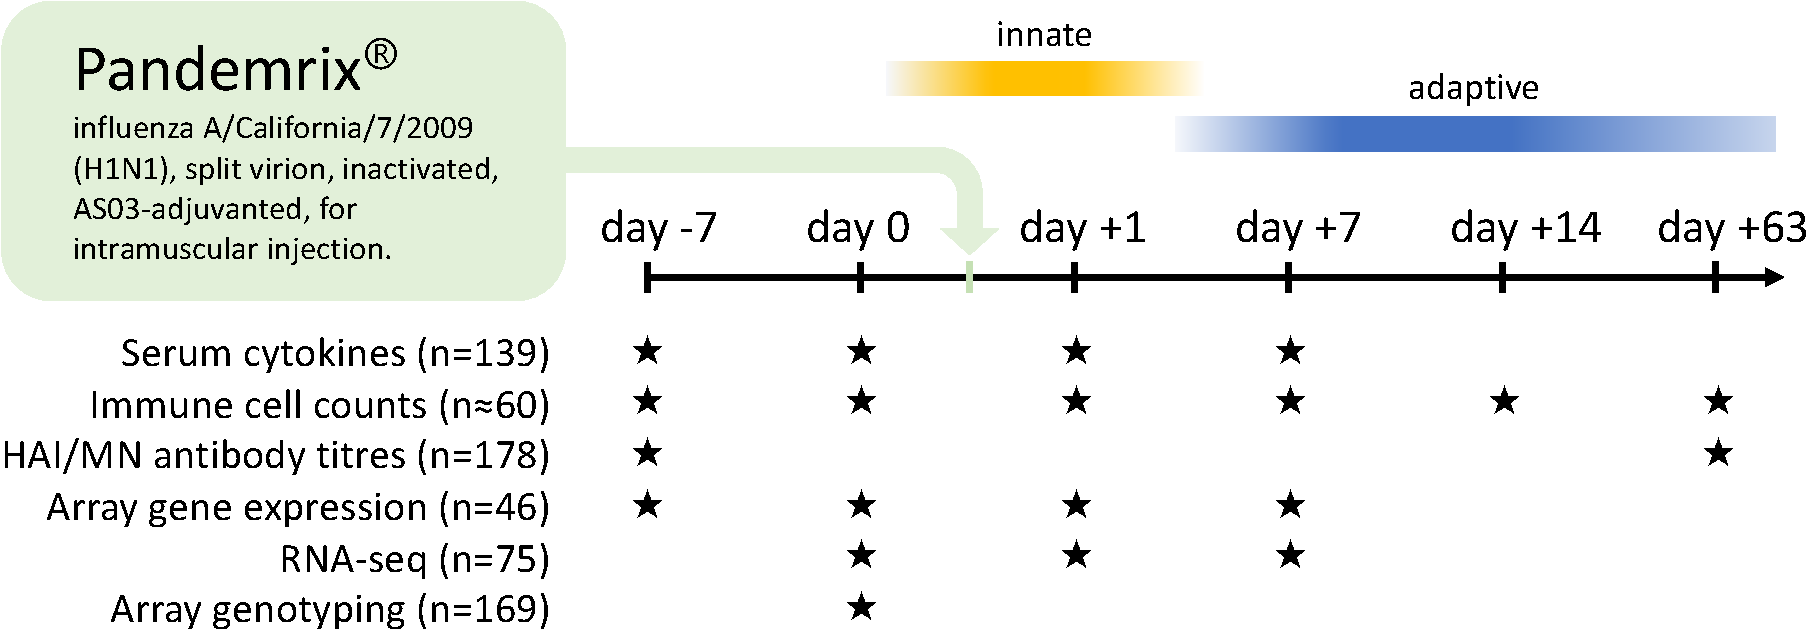
\includegraphics[width=1.0\textwidth]{mainmatter/figures/chapter_02/graphics_ashg19/hird_design-crop.pdf}
    \caption{Data types, timepoints, and sample sizes. Individuals were vaccinated after day 0 sampling. Antibodies to the vaccine strain were measured by \gls{HAI} and \gls{MN} assays. Array and \gls{RNAseq} gene expression measured in the \gls{PBMC} compartment.}
    \label{fig:hird_design}
\end{figure}

\subsection{Computing baseline-adjusted measures of antibody response}
\label{subsec:hird_dge_TRI}

In \autocite{sobolev2016AdjuvantedInfluenzaH1N1Vaccination}, Pandemrix responders were defined as individuals with $\ge$4-fold titre increases in either the \gls{HAI} or \gls{MN} assays.
This is a threshold for seroconversion set out by the U.S. Food and Drug Administration\autocite{foodanddrugadministration2007GuidanceIndustryClinical}, and is used in many studies of seasonal influenza vaccines\autocite{hagan2015SystemsVaccinologyEnabling}.
The responder status for 166 individuals with both \gls{HAI} and \gls{MN} titres available at baseline (day -7) and post-vaccination (day 63) were computed according to this definition.
\todo{atm I'm not using R/NR. wording here implys I am}
% \begin{outline}
% \1 Pre-process phenotypes
%     \2 Compute responder status (>= 4-fold in HAI or MN)
%     \2 Compute TRI (based on Bucasas 2009)
%         \3 “We related the change in titer between pre- and postvaccination measurements (response variable) to the prevaccination titer (explanatory variable) using a simple linear model”
%         \3 “We next determined the residuals from the above linear regressions and used them as the input values for the individual response scores.”
%         \3 “we standardized the residuals by dividing by the residual standard deviation for each component”
%             \4 Based on their axis ranges, it appears they are plotting log2(post)-log2(pre)), equivalently log2(post/pre), a.k.a. log2 fold-change; against log2(pre)
%             \4 Note that log2(post-pre) does not make sense mathematically, as post-pre may well be negative
%             \4 The negative relationship indicates lower initial titres are more amenable to high fold-change increases, which is exactly what TRI is designed to correct for
% \end{outline}
\todo{heterogeneity: well of course there was}
% TODO: here correct only for 2 things: dicot and RTM of change scores
However, \autocite{sobolev2016AdjuvantedInfluenzaH1N1Vaccination} noted there was heterogeneity in the baseline titres of non-responders, citing \enquote{glass ceiling} non-responders whose high baseline titres made the fixed 4-fold threshold hard to achieve.\todo{cite appropriate subfigures here}
% TODO: TRI is a residualised change score \url{https://www.tandfonline.com/doi/abs/10.1080/02732173.1991.9981960?journalCode=usls20}
\todo{change score is usually negatively correlated to baseline \autocite{clifton2019CorrelationBaselineScore}}
\todo{this is due to within-individual RTM , which is why we residualise}%\url{https://academic.oup.com/ije/article/34/1/215/638499#10889734}
\todo{the variable is not used as an inclusion/exclusion criterion for the study, otherwise regression to the mean will be strong} % https://rss.onlinelibrary.wiley.com/doi/full/10.1111/j.1740-9713.2011.00509.x
\todo{upend change score bit, the only thing we are concerned wtih here is clifton2019CorrelationBaselineScore}
% TODO: also cite https://academic.oup.com/ije/article/34/1/215/638499 : ANCOVA to adjust for regression to the mean
Dichotomisation of continuous response variables can also result in loss of statistical power \autocite{cohen1983CostDichotomization, fedorov2009ConsequencesDichotomization}.
% TODO: efficiency
% elaborate fully on why Dichot is bad here for the discussion: definition of response based on dichotomisation is inefficient and assumes a sharp change at the threshold

To address these concerns, I computed the \gls{TRI} as defined in \textcite{bucasas2011EarlyPatternsGene}.
For each assay, a linear regression was fit with the $\log_2{\text{day 63}/\text{day -7}}$ titre fold change as the response, and the $\log_2{\text{day -7}}$ baseline titre as the predictor.
The residuals from the two regressions were each standardized to zero mean and unit variance, then averaged.
The \gls{TRI} expresses a continuous measure of change in antibody titres across both assays post-vaccination, compared to individuals with a similar baseline titre, and remains comparable to the binary 4-fold change definition (\autoref{fig:hird_tri}).\todo{cite appropriate subfigures here, after adding proper subfigure labels}

\begin{figure}
    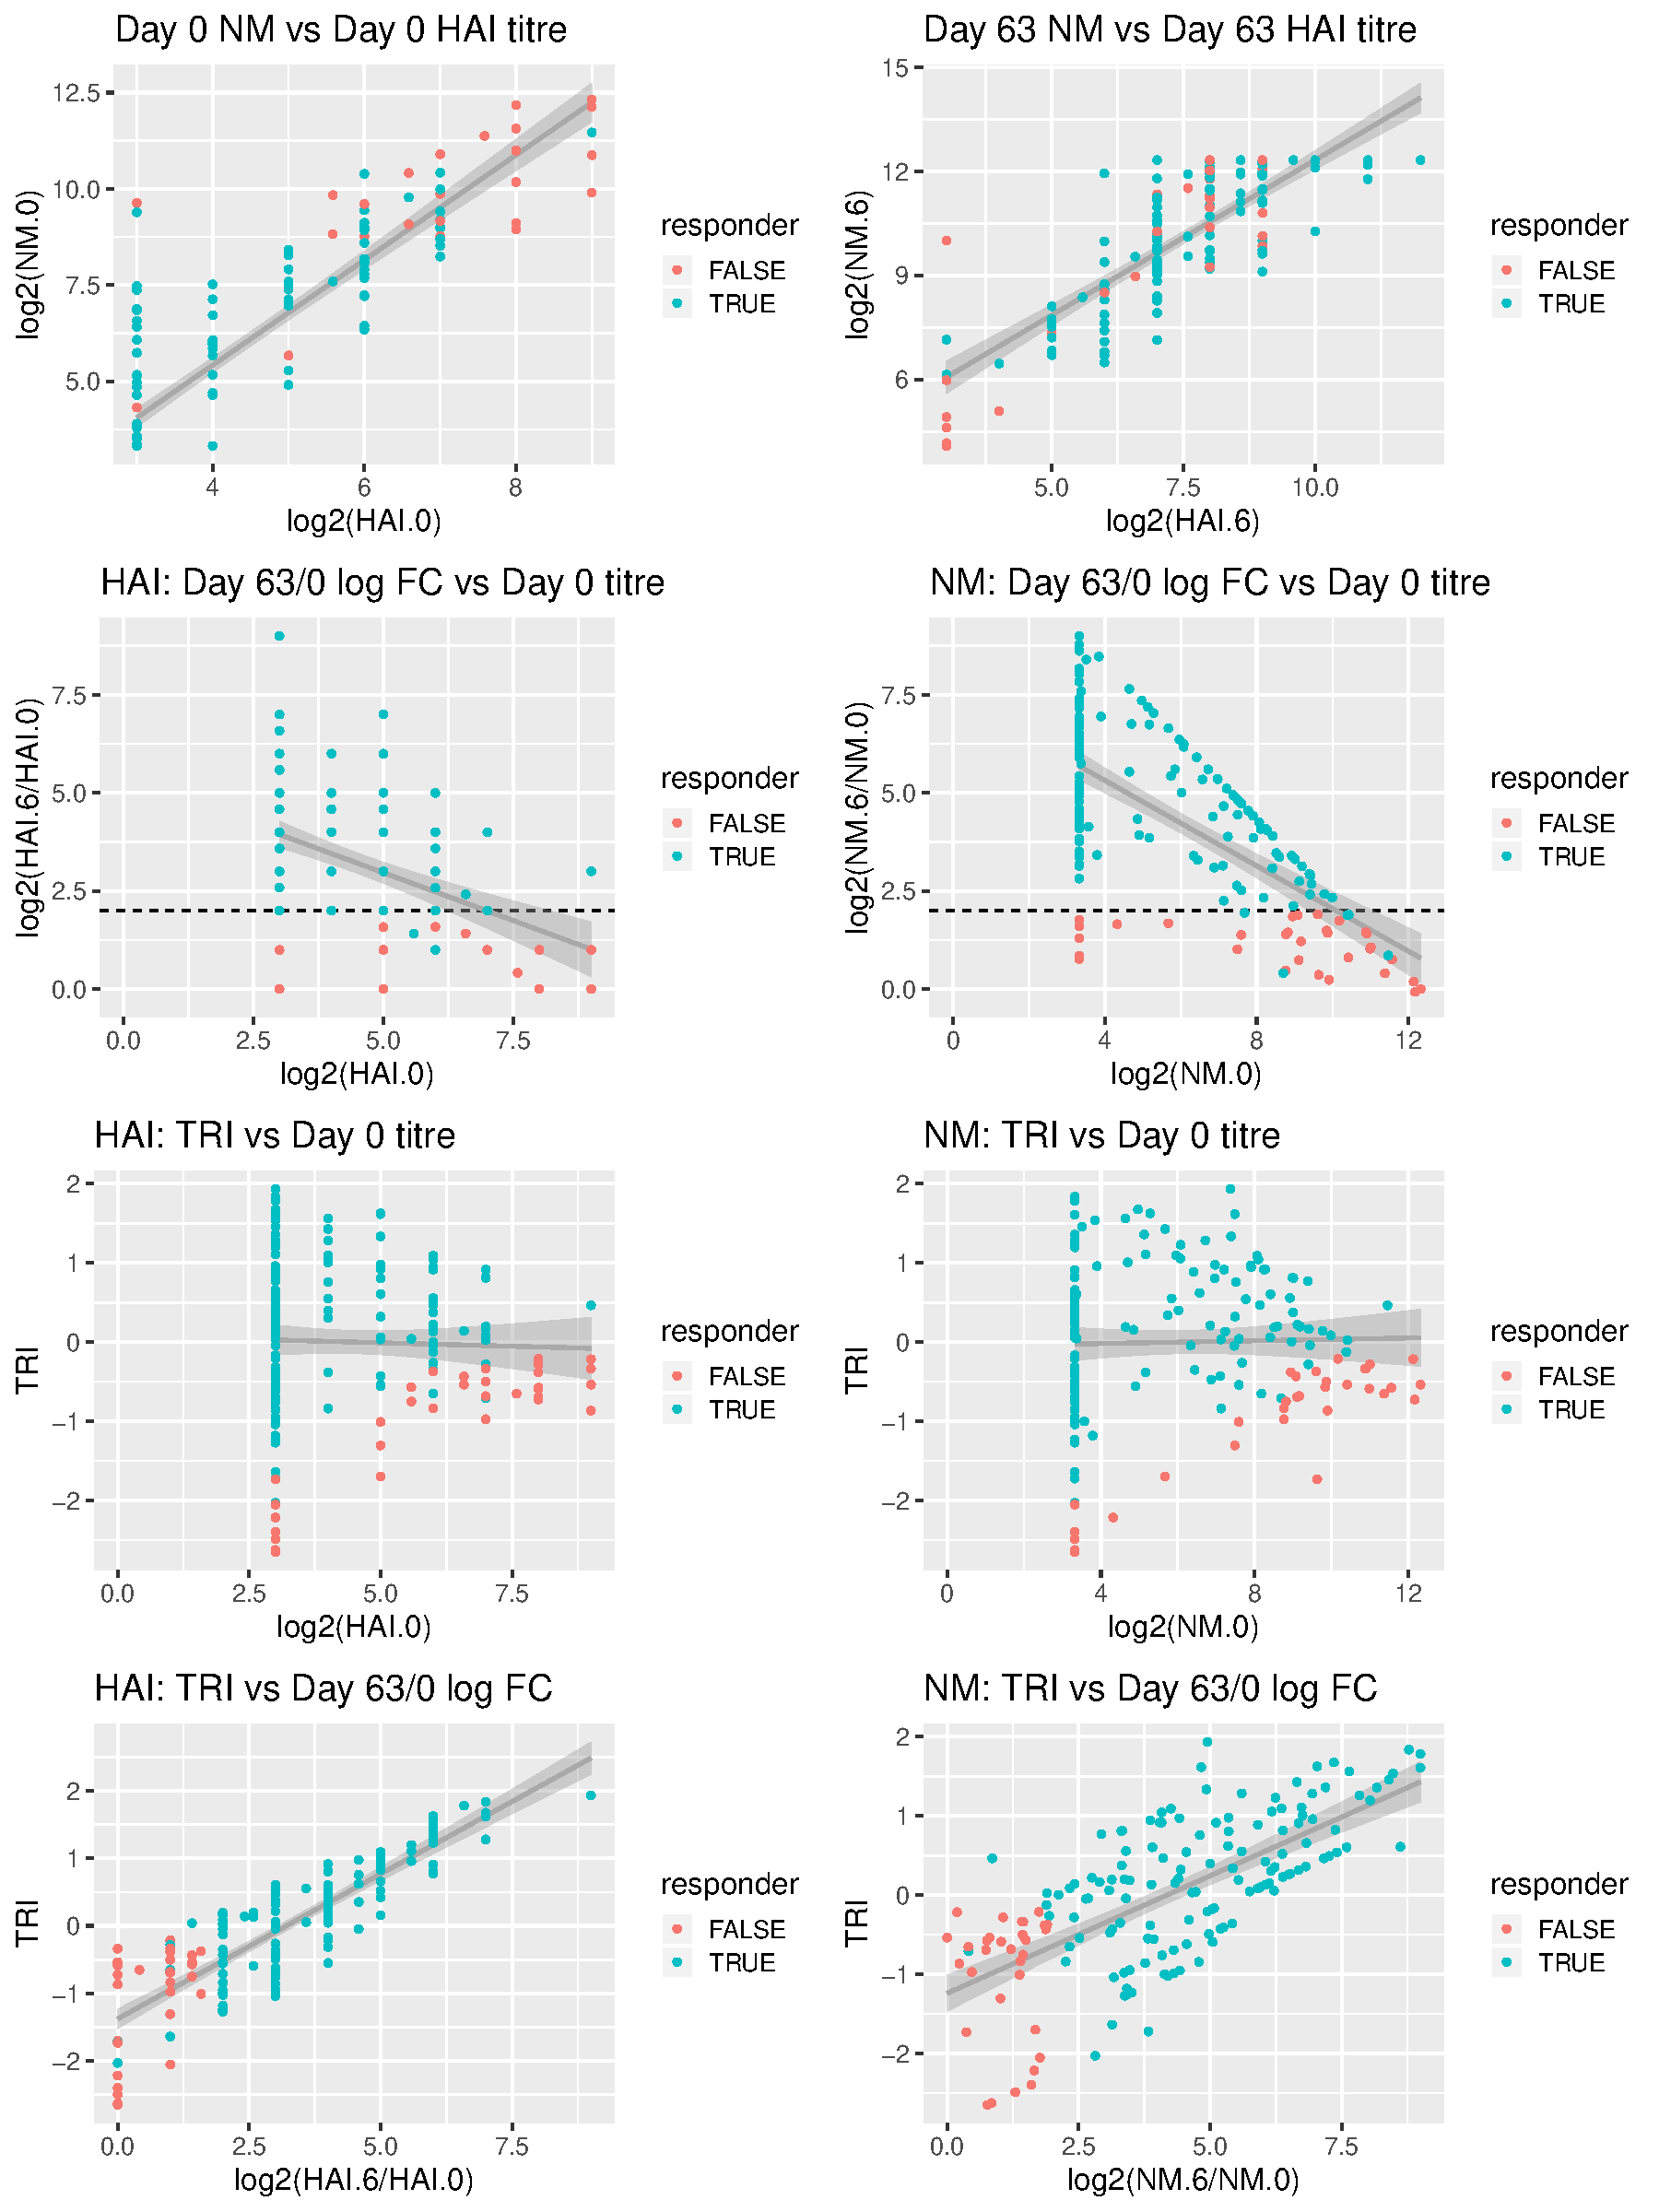
\includegraphics[width=1.0\textwidth]{mainmatter/figures/chapter_02/phenotype_data_setup.tri_comparison.pdf}
    \caption{Comparison of \gls{TRI} to \gls{HAI} (left column) and \gls{MN} (right column) titres and binary responder/non-responder status (colored) in 166 \gls{HIRD} individuals. Row 1: baseline titres are positively correlated to post-vaccination titres. Row 2: baseline titres are negatively correlated to fold change. Row 3: \gls{TRI} regresses out the correlation between baseline titre and response. Row 4: \gls{TRI} is still comparable in ordering to binary response status.}
    \label{fig:hird_tri}
\end{figure} 

Descriptive statistics for the 114 individuals with both gene expression and antibody titre data are presented in \autoref{tab:hird_table1}.
Although the proportion of responders between array (32/44) and \gls{RNAseq} (59/70) individuals is similar ($p = 0.1551$, Fisher's exact test), the variance of \gls{TRI} in array individuals is higher ($p = 0.0002098$, Levene's test), suggesting more extreme antibody response phenotypes are present (\autoref{fig:hird_phenotypes_by_platform}).
The cause of this is unknown, there is a possibility that individuals with more extreme phenotypes were prioritised for array transcriptomics in the original \gls{HIRD} study\footnote{Personal communication with authors.}.

\begin{table}[] 
 \centering 
 \caption{\textbf{Descriptive statistics for individuals with both expression and antibody data.} Values are count and percentage for categorial variables; mean and standard deviation for continuous variables. P values are for the comparison between platforms.}\label{tab:hird_table1}
 \begin{tabular}{ l c c c }
 \toprule
  &   &  \multicolumn{ 2 }{c}{ Platform }\\ 
  & Total & Array & \gls{RNAseq} \\ 
  & n = 114 & n = 44 & n = 70 \\ 
  \midrule
 Gender &   &   &  \\ 
 \hspace{6pt}    F & 72 (63.2\%) & 27 (61.4\%) & 45 (64.3\%)\\ 
 \hspace{6pt}    M & 42 (36.8\%) & 17 (38.6\%) & 25 (35.7\%)\\ 
 Age at vaccination (years)  &   &   &  \\ 
 \hspace{6pt}   & 29.2 (11.8) & 32.9 (14.1) & 26.8 (9.4)\\ 
 Ancestry (self-reported) &   &   &  \\ 
 \hspace{6pt}    Asian & 14 (12.3\%) & 5 (11.4\%) & 9 (12.9\%)\\ 
 \hspace{6pt}    Black/African & 9 (7.9\%) & 4 (9.1\%) & 5 (7.1\%)\\ 
 \hspace{6pt}    Caucasian & 82 (71.9\%) & 33 (75\%) & 49 (70\%)\\ 
 \hspace{6pt}    Latin American & 2 (1.8\%) & 1 (2.3\%) & 1 (1.4\%)\\ 
 \hspace{6pt}    Mixed & 5 (4.4\%) & 1 (2.3\%) & 4 (5.7\%)\\ 
 \hspace{6pt}    Other - Arab & 1 (0.9\%) & 0 (0\%) & 1 (1.4\%)\\ 
 \hspace{6pt}    White Other & 1 (0.9\%) & 0 (0\%) & 1 (1.4\%)\\ 
 log2 day -7 HAI  &   &   &  \\ 
 \hspace{6pt}   & 4.4 (1.8) & 4.2 (1.6) & 4.5 (1.9)\\ 
 log2 day 63 HAI  &   &   &  \\ 
 \hspace{6pt}   & 7.6 (1.8) & 7.4 (2.2) & 7.6 (1.5)\\ 
 log2 HAI fold change  &   &   &  \\ 
 \hspace{6pt}   & 3.2 (1.9) & 3.2 (2.4) & 3.1 (1.6)\\ 
 log2 day -7 MN  &   &   &  \\ 
 \hspace{6pt}   & 6.2 (2.8) & 5.4 (2.4) & 6.6 (3.0)\\ 
 log2 day 63 MN  &   &   &  \\ 
 \hspace{6pt}   & 10.4 (2.0) & 9.5 (2.2) & 10.9 (1.6)\\ 
 log2 MN fold change  &   &   &  \\ 
 \hspace{6pt}   & 4.2 (2.3) & 4.1 (2.6) & 4.3 (2.1)\\ 
 Responder (binary definition) &   &   &  \\ 
 \hspace{6pt}    FALSE & 23 (20.2\%) & 12 (27.3\%) & 11 (15.7\%)\\ 
 \hspace{6pt}    TRUE & 91 (79.8\%) & 32 (72.7\%) & 59 (84.3\%)\\ 
 TRI &   &   &  \\ 
 \hspace{6pt}   & -0.0 (0.9) & -0.2 (1.2) & 0.1 (0.7)\\ 
 \bottomrule
 
 \end{tabular}
 \end{table}


\begin{figure}
    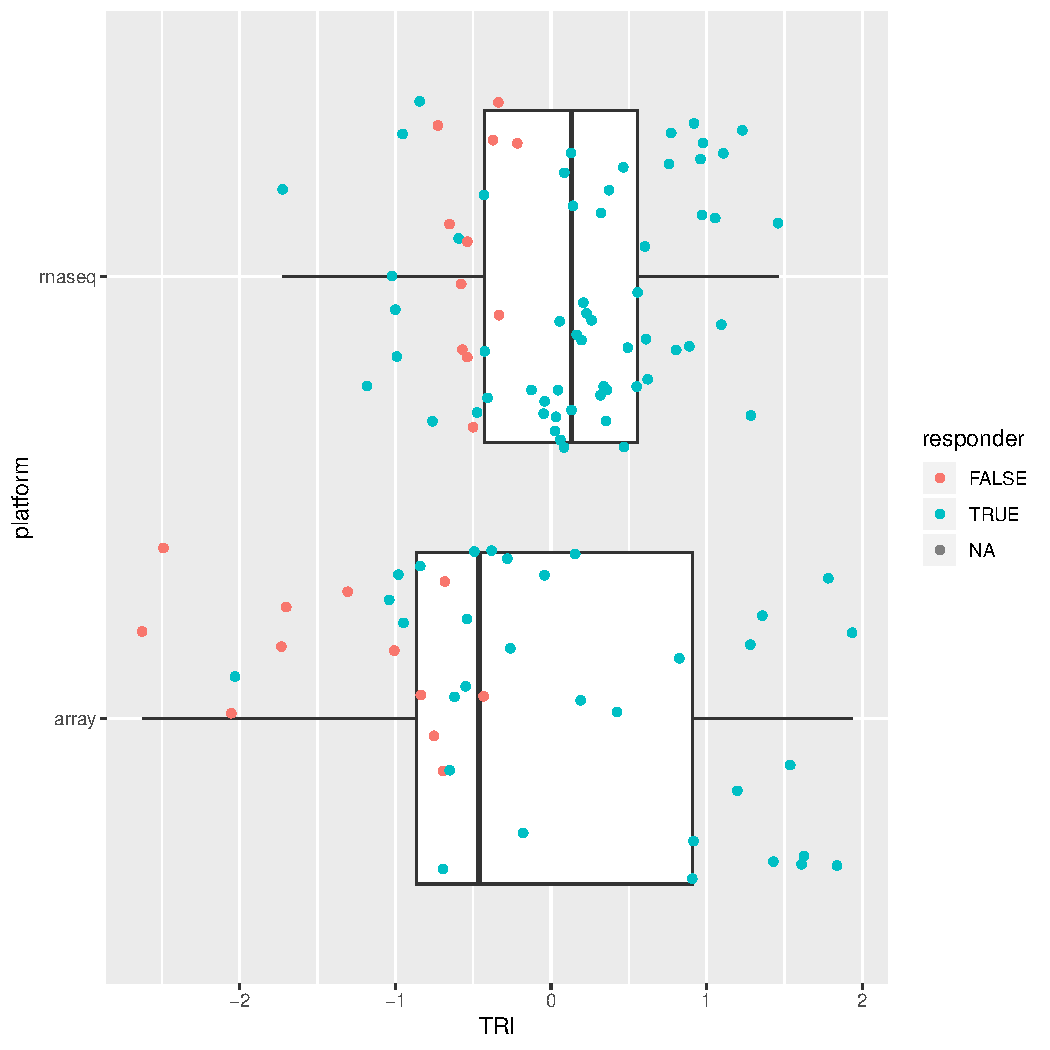
\includegraphics[width=1.0\textwidth,page=1]{mainmatter/figures/chapter_02/compare_phenotype_by_platform.pheno_boxplots.pdf}
    \caption{Distribution of \gls{TRI}, stratified by platform used to measure expression.}
    \label{fig:hird_phenotypes_by_platform}
\end{figure}

\subsection{Genotype data generation}

\todo{Add to collab note that extractions were done at KCL}
DNA was extracted from frozen blood using the Blood and Tissue DNeasy kit (Qiagen), and genotyping was performed using on the Infinium CoreExome-24 BeadChip (Illumina).
In total, 192 samples from 176 individuals in the HIRD cohort were genotyped at 550601 markers, including replicate samples submitted for individuals where extracted DNA concentrations were low.

\subsection{Genotype data preprocessing}
\label{subsec:hird_dge_genotype_preproc}

Using PLINK (v1.90b3w), genotype data underwent the following quality control procedures to remove poorly genotyped samples and markers:
max marker missingness across samples $< 5\%$, 
max sample missingness across markers $< 1\%$, 
max marker heterozygosity rate within 3 standard deviations of the mean (threshold selected visually to exlude outliers, \autoref{fig:hird_genotype_sample_hetRate_missingness}),
% TODO: recheck if this is really max marker heterozygosity rate, not sample rate
% TODO: add discordant sex mismatch to indicate possible sample swaps, distribution of F estimates
% The HWE threshold should depend on the multi-ethnicity of the cohort
% \todo{see}
% https://www.nature.com/articles/nrg2344
% Once armed with a set of called genotypes, the final phase of quality control beckons. Experience has shown that most SNPs showing extreme departures from Hardy–Weinberg equilibrium (HWE) in controls can be safely discarded1, although lesser (but nevertheless quite marked) departures are to be expected under the null hypothesis, given the number of tests performed. Appropriate thresholds for any given study will depend on the sample size and overall data quality, and might best be defined by using the observed distribution of HWE statistics (the WTCCC used this approach to set a threshold at an exact p < 5.7 × 10−7 in controls)1. In any event, HWE is an imprecise tool for quality control purposes. Tests of departure from HWE are underpowered for the detection of genotyping error75,76, whereas overenthusiastic use of HWE as a quality criterion can prove to be counterproductive given that modest disequilibrium (in cases particularly) can be a signature of true association.
removal of markers that deviate from \gls{HWE} (\texttt{-{}-hwe} option, $\text{p} < 0.00001$).
% TODO
% We exclude markers that show extensive deviation from Hardy-Weinberg equilibrium (HWE) because
%   this can be indicative of a genotyping or genotype-calling error. However,
%   deviations from HWE may also indicate selection; accordingly,
%   if a case sample shows deviations from HWE at loci associated with disease,
%   it would obviously be counterproductive to remove these loci from further investigation.
%   Therefore, only control samples should be used when testing for deviations for HWE.
  

\begin{figure}
    \includegraphics[width=1.0\textwidth,page=2]{mainmatter/figures/chapter_02/coreex_eQTLflu_20171204.gencall.smajor.impute_sex.qc2.pdf}
    \caption{Sample filters for missingness and heterozygosity rate. Samples outside the central rectangle were excluded.}
    \label{fig:hird_genotype_sample_hetRate_missingness}
\end{figure}

To exclude highly-related individuals and deduplicate replicate samples, pairwise kinship coefficients were computed on \gls{MAF} $< 0.05$ pruned genotypes using KING (v1.4).
For each pair of samples with pairwise kinship coefficient $> 0.177$ (first-degree relatives or closer), the sample with lower marker missingness was selected.

After filtering, 169 samples and 549414 markers remained.

\subsection{Computing genotype \glsfmtlongpl{PC} as covariates for ancestry}
\label{subsec:hird_dge_genotype_pc}

% TODO: read
% Efficient toolkit implementing best practices for principal component analysis of population genetic data

As shown in \autoref{tab:hird_table1}, the \gls{HIRD} cohort is multi-ethnic, hence there is potential for confounding by population structure (sample structure due to genetic background) and genetic association studies \autocite{price2006PrincipalComponentsAnalysis,eu-ahsunthornwattana2014ComparisonMethodsAccount}.
Large-scale population structure explains variation in gene expression \autocite{brown2018ExpressionReflectsPopulation}, so including population structure as covariates can increase power.
Treating HapMap 3 samples \autocite{theinternationalhapmap3consortium2010IntegratingCommonRare} as a reference population where the major axes of variation in genotypes are likely to be ancestry, \gls{PCA} was performed using smartpca (v8000) on \gls{LD}-pruned genotypes (\texttt{PLINK -{}-indep-pairwise 50 5 0.2}).
% https://journals.plos.org/plosone/article?id=10.1371/journal.pone.0093766
% TODO: Prior to PCA, thinning of the SNPs by LD and removal of regions with known high LD or other artefacts such as inversions have been recommended [1], [15], as high correlations between the SNPs can distort the resulting eigenvectors.
% TODO
% price2006PrincipalComponentsAnalysis supp note
% Linkage disequilibrium and choice of markers. Genome-wide data sets containing hundreds of thousands of markers are likely to exhibit substantial linkage disequilibrium (LD) between markers, even in the case of markers chosen to optimally tag all variation in the genome. Thus,
% Page 6inferring population structure from the set of all markers has two potential problems. The first problem is that, due to varying levels of LD, some regions will have more redundant markers than others and will thus be overrepresented. The second problem is that strong LD at a given locus which affects many markers could result in an axis of variation which corresponds to genetic variation specifically at that locus, rather than to genome-wide ancestry. Nonetheless, we recommend inferring population structure using all markers. This recommendation is based on an analysis of HapMap8 data which suggests that these potential problems will not affect results in practice, even on a data set with over 3 million markers
% TODO: why exclude long range/prune
% https://www.nature.com/articles/ejhg201348
% Very strong and/or long-range LD at a particular locus can even result in PCs that only reflect genetic variation at that specific locus.6, 7
% We thus conclude that both excluding long-range LD regions and LD pruning are necessary when studying a relatively small population, which may consist of overlapping subpopulations.
\gls{HIRD} sample \glspl{PC} were computed by projection onto the HapMap 3 \gls{PCA} eigenvectors.
% TODO: this vs in-sample pca
% TODO http://www.biostatgen.org/wp-content/uploads/2018/09/bby081.pdf % If we assume that the correlation structure itselfdiffers between cases and controls, then it makes sense to do thePCA on controls and then project its results on cases as discussedin [71]. However, if we assume that the structure itself may bethe same, but just the factor values are different, then we coulduse the entire group for the PCA to have a larger sample sizeand obtain more stable results.
% TODO: https://www.ncbi.nlm.nih.gov/pmc/articles/PMC6007879/#!po=31.2500
% if there may be related, prefer projection:
% Principal Components Analysis with Related individuals (PC-AiR) [Conomos, et al. 2015] infers PS in the presence of related individuals. This method identifies an unrelated subset of individuals that represents the ancestral diversity of the sample and computes PCs in this subset and projects PCs onto the remainder of the sample.
For non-genotyped individuals, \gls{PC} values were imputed as the mean value for all genotyped individuals with the same self-reported ancestry.
The top \glspl{PC} separate samples of European, African and Asian ancestry (\autoref{fig:hird_genotype_pca_withHapmap}), hence these \glspl{PC} can be used as continuous covariates for ancestry downstream.
\todo{Add Tracy-Widom statistics for PCs to justify later choice of 4 PCs for covariates}
% TODO: https://journals.plos.org/plosgenetics/article?id=10.1371/journal.pgen.0020190
\todo{nicer version, copy the peer code, facet the hird and hapmap samples}

\begin{figure}
    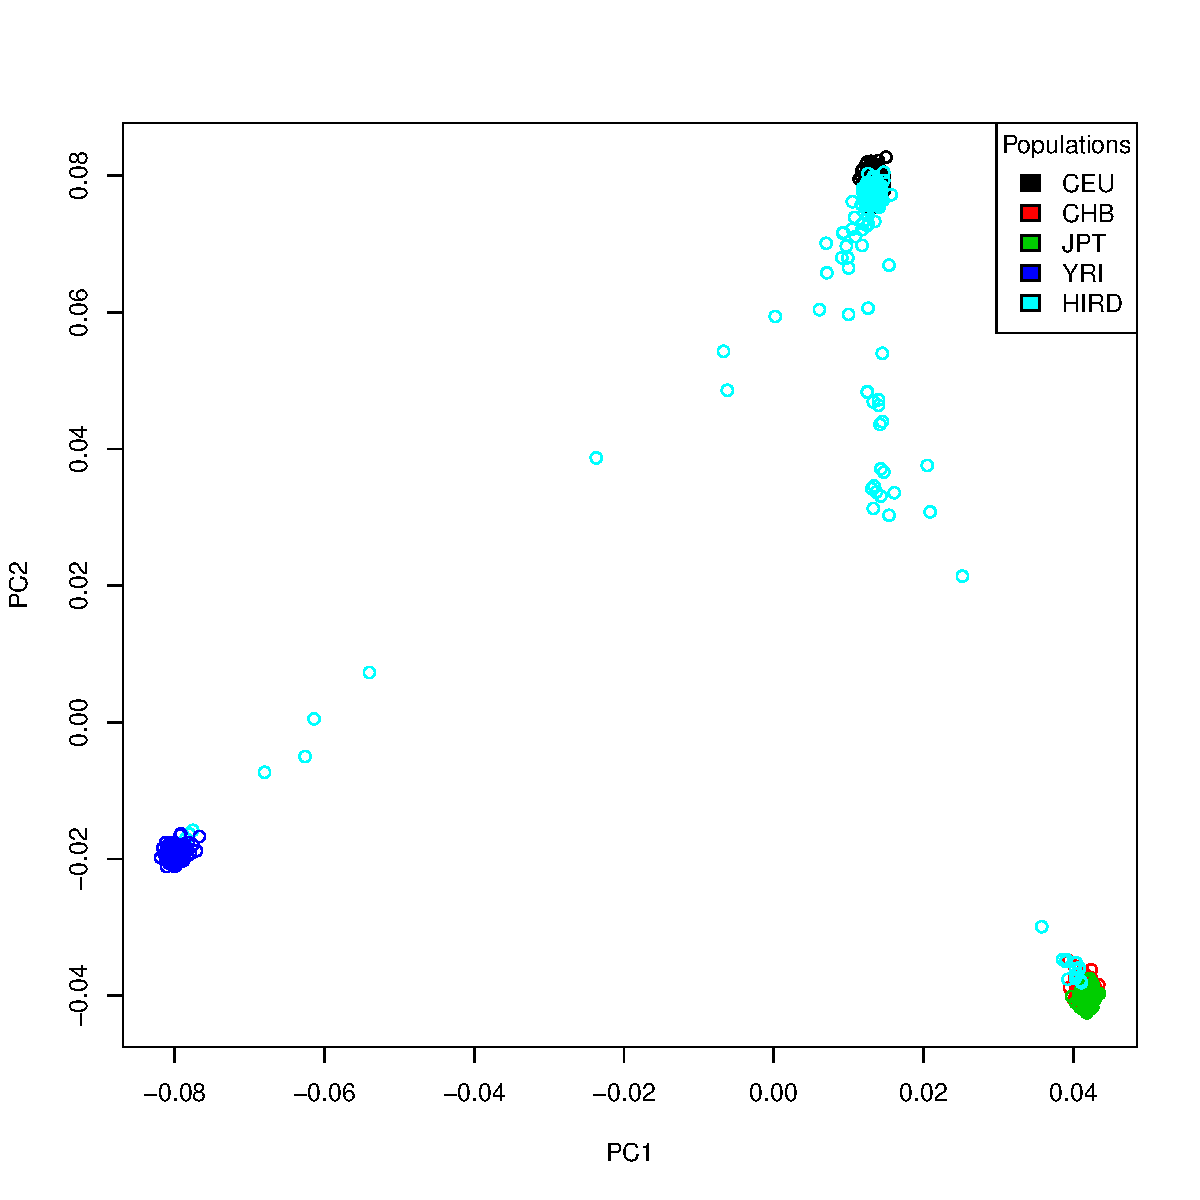
\includegraphics[width=1.0\textwidth]{mainmatter/figures/chapter_02/coreex_eQTLflu_20171204.gencall.smajor.impute_sex.qc3.pruned.hapmap_merged.flipped.pca.evec.pdf}
    \caption{\gls{HIRD} samples (cyan) projected onto \gls{PC}1 and \gls{PC}2 axes defined by \gls{PCA} of HapMap 3 samples. The first two \glspl{PC} separate European (CEU, upper-right) from Asian (CHB and JPT, lower-right) and African (YRI, lower-left) individuals.}
    \label{fig:hird_genotype_pca_withHapmap}
\end{figure}

\subsection{\glsfmtshort{RNAseq} data generation}

Total RNA was extracted from \glspl{PBMC} using the Qiagen RNeasy Mini kit, with on-column DNase treatment.
RNA integrity was checked on the Agilent Bioanalyzer and mRNA libraries were prepared with the KAPA Stranded mRNA-Seq Kit (KK8421), which uses poly(A) selection.
% 7 lanes x 3 plates
To avoid confounding of timepoint and batch effects from pooling, samples were pooled by library prep plate, ensuring libraries from all timepoints of an individual were in the same pool, and then sequenced across multiple lanes as technical replicates (HiSeq 4000, 75bp paired-end).

% To get to cram files:
% From .cram headers:
% 1.	The NextSeq, HiSeq, and NovaSeq Sequencing Systems generate raw data files in binary base call (BCL) format.
% 1.1.	HiSeq Sequencing Control Software (SCS), version HD 3.4.0.38, used for basecalling
% 2.	biobambam2/bamadapterfind: bamdapterfind scans a BAM file for contaminations by sequencing adapters.
% 3.	bambi decode: decode a multiplexed bam file
% 4.	bwa sampe (alignment using BWA-backtrack): alignment to phiX, which is then merged with the original bam
% 5.	pb_calibration/spatial_filter: Identify regions with spatially correlated errors e.g. bubbles, (from aligned BAM files where the read name can be parsed for spatial location) and allow filtering out or marking of the BAM fail bit for reads in those regions.
% 6.	Alignment with tophat 2.0.14
% 6.1.	 --keep-fasta-order --no-sort-bam --output-dir tophat_out_24165_1#10 --mate-inner-dist 100 --num-threads=8 --library-type=fr-firststrand --no-coverage-search --microexon-search --transcriptome-index=/lustre/scratch117/core/sciops_repository/transcriptomes/Homo_sapiens/ensembl_83_transcriptome/GRCh38_15_plus_hs38d1/tophat2/GRCh38_15_plus_hs38d1.known/lustre/scratch117/core/sciops_repository/references/Homo_sapiens/GRCh38_15_plus_hs38d1/all/bowtie2/Homo_sapiens.GRCh38_15_plus_hs38d1.fa
% 7.	Some sort of duplicate marking and filtering (?) using some combination of:
% 7.1.	biobambam/bamsormadup: parallel sorting and duplicate marking
% 7.2.	uk.ac.sanger.npg.picard.AlignmentFilter
% 7.3.	biobambam/bamstreamingmarkduplicates
% 8.	Write .cram files using scramble (cram is a reference-based compression)
% 8.1.	/lustre/scratch117/core/sciops_repository/references/Homo_sapiens/GRCh38_15_plus_hs38d1/all/fasta/Homo_sapiens.GRCh38_15_plus_hs38d1.fa
% 9.	NOTE: Note lots of intermediate biobambam 2.0.76 and scramble processing steps, not all are listed.

\todo{Can add other fastqc plots e.g. kmers, overrepresented seqs, seq length}
% Genomic origin of reads and gene end biases were assessed using Qualimap, after aligning the reads to the human GRCh38_15_plus_hs38d10 reference transciptome using tophat2.
\gls{RNAseq} quality metrics were assessed using FASTQC\footnote{\url{https://www.bioinformatics.babraham.ac.uk/projects/fastqc/}} and Qualimap\autocite{okonechnikov2015QualimapAdvancedMultisample}, then visualised with MultiQC\autocite{ewels2016MultiQCSummarizeAnalysis}.
% See log 2017-11-20 for fastqc discussion
Sequence quality was high (\autoref{fig:hird_fastqc_seqQual}), and duplication levels were low (\autoref{fig:hird_fastqc_seqDupe}).
The unimodal GC-content distribution suggested negligible levels of non-human contamination (\autoref{fig:fastqc_gc}).

\begin{figure}
	\centering
	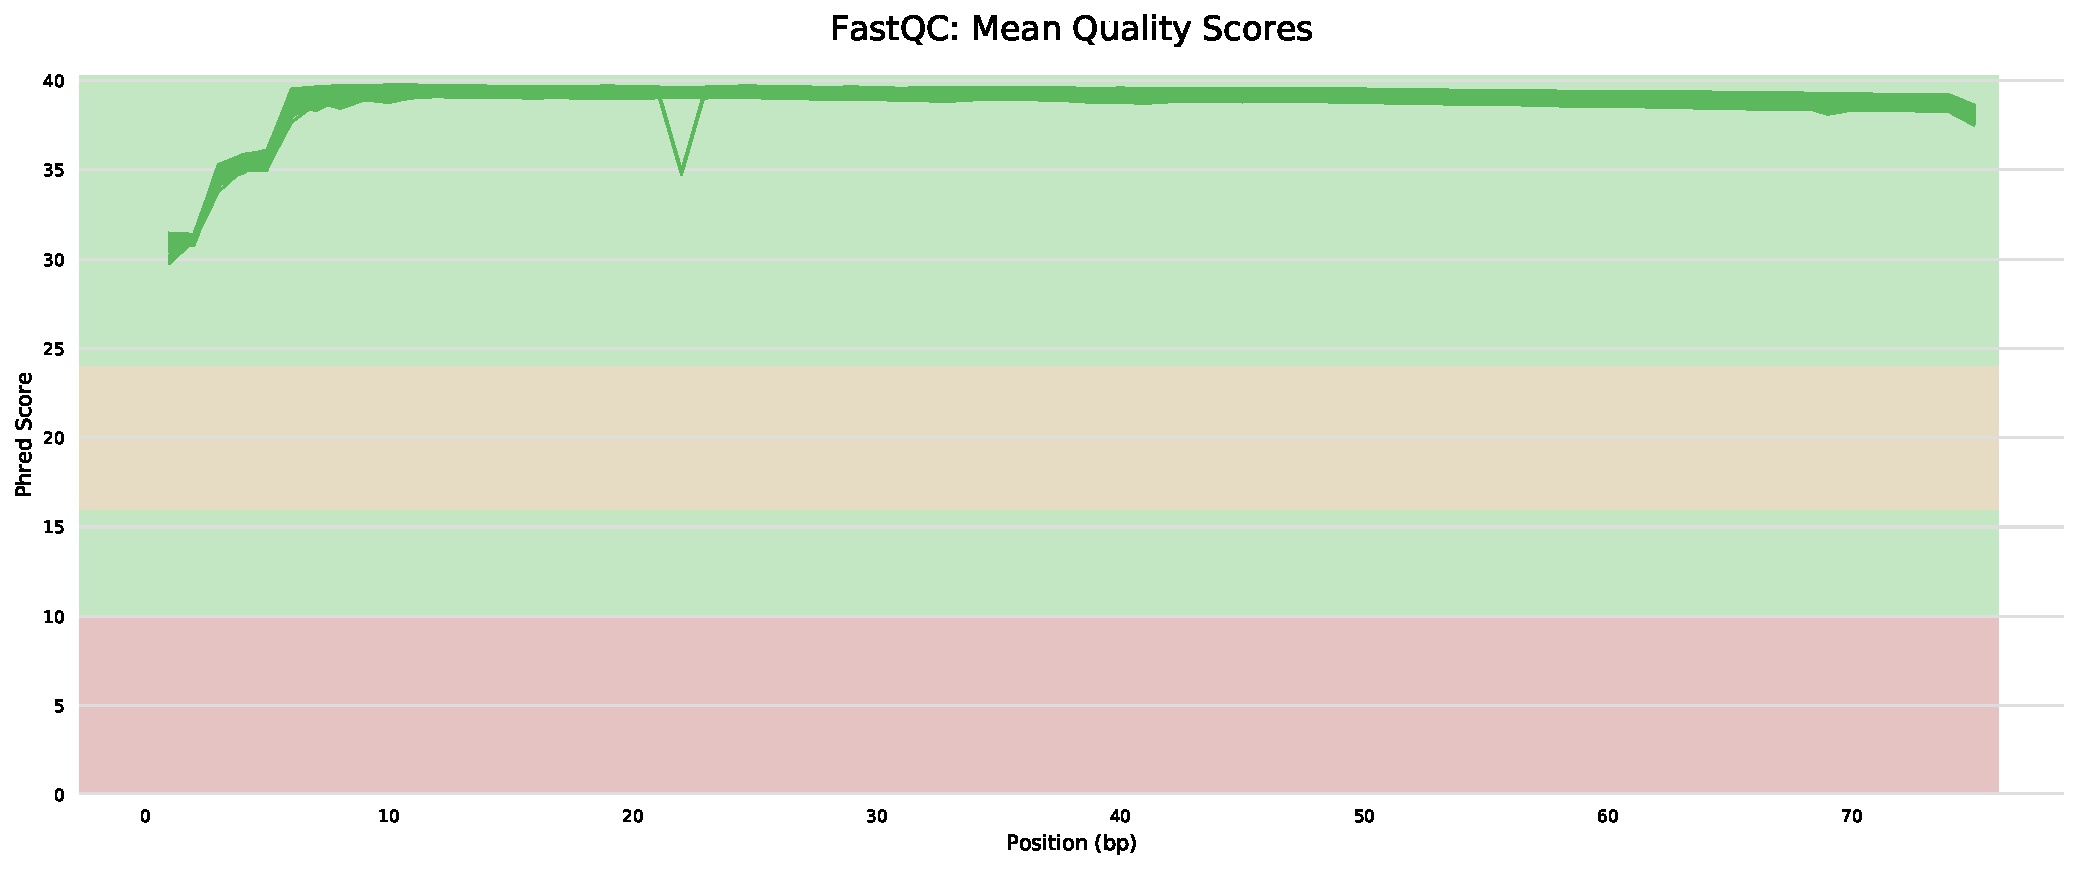
\includegraphics[width=\textwidth]{mainmatter/figures/chapter_02/graphics_firstYearReport/fastqc/mqc_fastqc_per_base_sequence_quality_plot_1.pdf}
    \caption{FastQC sequence quality versus read position for \gls{HIRD} \gls{RNAseq} samples.}
	\label{fig:hird_fastqc_seqQual}
\end{figure}

\begin{figure}
	\centering
	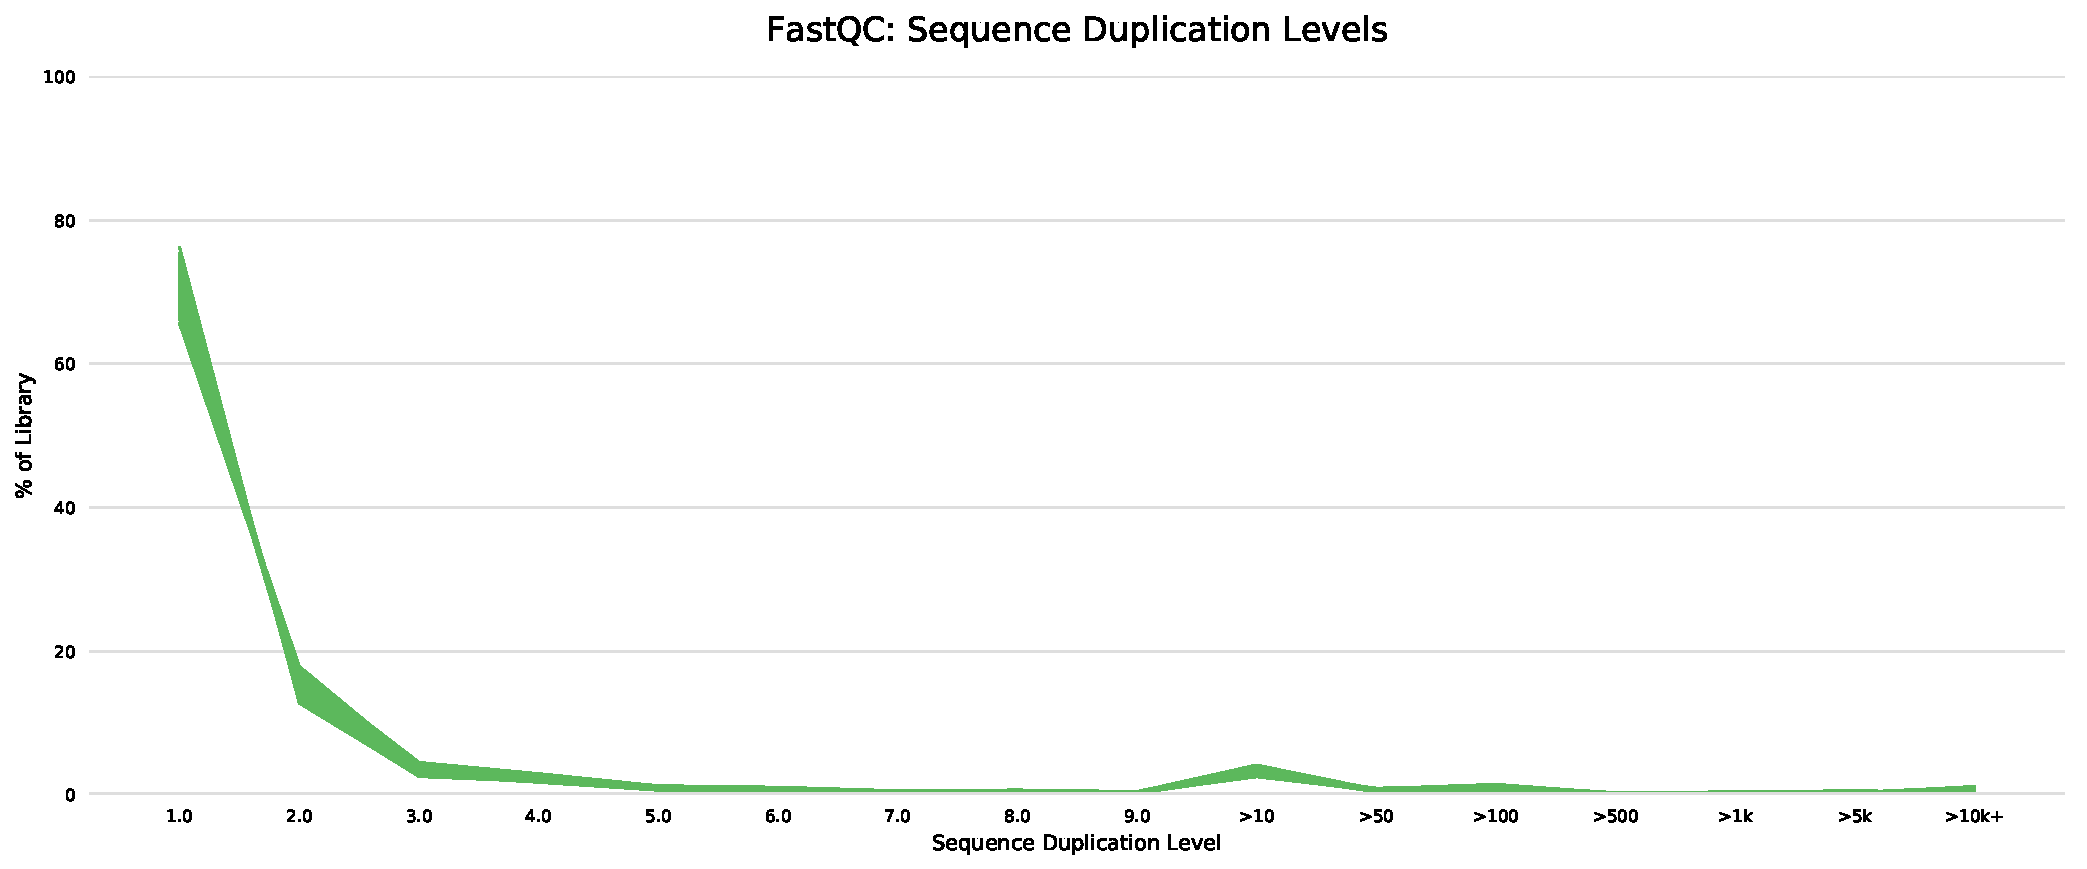
\includegraphics[width=\textwidth]{mainmatter/figures/chapter_02/graphics_firstYearReport/fastqc/mqc_fastqc_sequence_duplication_levels_plot_1.pdf}
	\caption{FastQC sequence duplication levels for \gls{HIRD} \gls{RNAseq} samples.}
	\label{fig:hird_fastqc_seqDupe}
\end{figure}

\begin{figure}
	\centering
	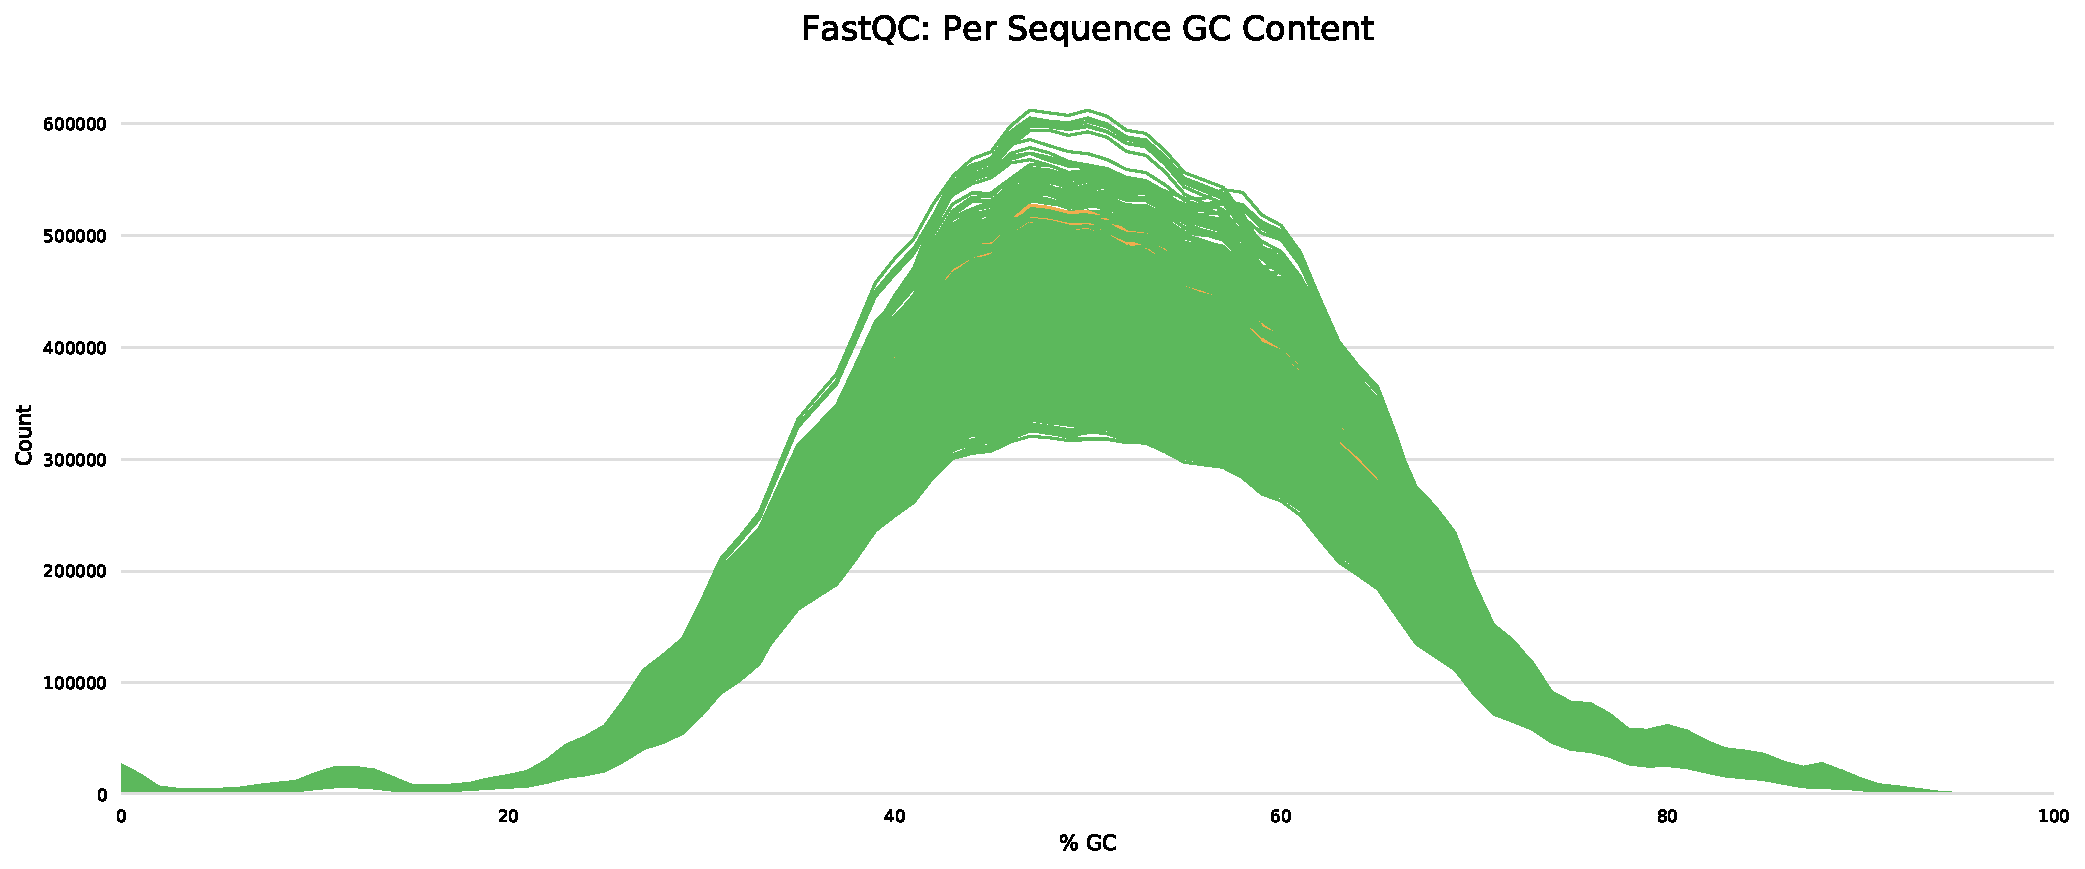
\includegraphics[width=\textwidth]{mainmatter/figures/chapter_02/graphics_firstYearReport/fastqc/mqc_fastqc_per_sequence_gc_content_plot_Counts.pdf}
	\caption{FastQC GC profile for \gls{HIRD} \gls{RNAseq} samples.}
	\label{fig:fastqc_gc}
\end{figure}

\subsection{\glsfmtshort{RNAseq} quantification and filtering}
\label{subsec:hird_dge_rnaseq_quantAndFilter}

% 1.	Quantification (Salmon --libType ISR, which is equiv to TopHat -fr-firststrand with paired end data)
% 1.1.	Used index /lustre/scratch117/core/sciops_repository/transcriptomes/Homo_sapiens/ensembl_83_transcriptome/GRCh38_15_plus_hs38
% 1.1.1.	This is GRCh38.p5, Dec 2017, v83; with additional hs38d1: Decoy version 1 for GRCh38
% 1.1.2.	Contains ENST transcript ids
% 1.2.	Output quantifies transcripts in terms of: TPM — This is salmon’s estimate of the relative abundance of this transcript in units of Transcripts Per Million (TPM). TPM is the recommended relative abundance measure to use for downstream analysis.
% 1.2.1.	https://haroldpimentel.wordpress.com/2014/05/08/what-the-fpkm-a-review-rna-seq-expression-units/ TPM = (count/effectiveLength) / sumOverAllTranscripts(count/effectiveLength)
% 1.3.	Note Salmon also takes into account: EffectiveLength — This is the computed effective length of the target transcript. It takes into account all factors being modeled that will effect the probability of sampling fragments from this transcript, including the fragment length distribution and sequence-specific and gc-fragment bias (if they are being modeled).
% 2.	Gene-level regeneration of counts (tximport)
% 2.1.	“generate estimated counts using abundance estimates scaled up to library size (scaledTPM)”
% 2.1.1.	Note, we do not scale for gene length, that would be lengthScaledTPM. Hence the generated counts remain length-corrected.
% 2.2.	Summarizes using a mapping of ENST to ENSG, generated from /lustre/scratch117/core/sciops_repository/transcriptomes/Homo_sapiens/ensembl_83_transcriptome/GRCh38_15_plus_hs38d1/gtf/ensembl_83_transcriptome-GRCh38_15_plus_hs38d1.gtf
% 2.3.	Counts from all lanes of a sample are summed
% 3.	GC bias, length bias, mappability
% 3.1.	Length bias only affects RNAseq: somewhat alleviated by Salmon using effective length
% 3.2.	GC bias affects both technologies: somewhat alleviated by Salmon using effective length (see the salmon paper)
% NOTE:
% 3.3.	Mappability has not been considered
\todo{add software versions}
% NOTE: Salmon is not pseudo-alignment: "Unlike pseudoalignment, Salmon’s lightweight mapping procedure tracks, by default, the position and orientation of all mapped fragments."
% TODO: https://www.ncbi.nlm.nih.gov/pmc/articles/PMC6042521/ Limitations of alignment-free tools in total RNA-seq quantification
Reads were quantified against the Ensembl reference transcriptome (GRCh38) using Salmon\autocite{patro2017SalmonProvidesFast} in quasi-mapping-based mode, 
which internally corrects for transcript length and GC composition by computing an effective length for each transcript.
% https://www.biostars.org/p/304552/
% TODO: check, this should be done after converting TPM to counts with tximport? summing TPMs doesn't make sense
To combine technical replicates, as the sum of Poisson distributions remains Poisson-distributed, counts for technical replicates were summed for each sample.
% Also see:
%
% https://genomebiology.biomedcentral.com/articles/10.1186/s13059-016-0881-8
% "While some authors will argue that as few as five million mapped reads are sufficient to quantify accurately medium to highly expressed genes in most eukaryotic transcriptomes, others will sequence up to 100 million reads to quantify precisely genes and transcripts that have low expression levels [7]."
%
% https://genome.ucsc.edu/ENCODE/protocols/dataStandards/ENCODE_RNAseq_Standards_V1.0.pdf
% 2. Sequencing depth.
% The amount of sequencing needed for a given sample is determined by the goals of the experiment and the nature of the RNA sample.
% Experiments whose purpose is to evaluate the similarity between the transcriptional profiles of two polyA+ samples may require only modest depths of sequencing (e.g. 30M pair-end reads of length > 30NT, of which 20-25M are 3mappable to the genome or known transcriptome, Experiments whose purpose is discovery of novel transcribed elements and strong quantification of known transcript isoforms requires more extensive sequencing.
% The ability to detect reliably low copy number transcripts/isoforms depends upon the depth of sequencing and on a sufficiently complex library.
% For experiments from a typical mammalian tissue or in which sensitivity of detection is important, a minimum depth of 100-200 M 2 x 76 bp or longer reads is currently recommended.
The mean number of mapped read pairs per sample after summing was 27.09 million read pairs (range 20.24-39.14 million), representing a mean mapping rate of 80.73\% (range 75.57-90.10\%), comfortably within sequencing depth recommendations for \gls{DGE} experiments\autocite{liu2014RNAseqDifferentialExpression}.
% TODO: add exact rule of thumb diminishing returns for DGE after 10M aligned reads
Relative transcript abundances were summarised to Ensembl gene-level count estimates using tximport (scaledTPM method) to improve statistical robustness and interpretability\autocite{soneson2016DifferentialAnalysesRNAseq}.

% TODO:
% why use length scaled tpm, not salmon counts directly?
% We could alternatively generate counts from abundances, using the argument countsFromAbundance, scaled to library size, "scaledTPM", or additionally scaled using the average transcript length, averaged over samples and to library size, "lengthScaledTPM". Using either of these approaches, the counts are not correlated with length, and so the length matrix should not be provided as an offset for downstream analysis packages.

% TODO
% Two main biases are library composition and feature length in RNAseq
% TPM would be for within sample norm for both
% no+use length offset, or scaledTPM, or lengthScaledTPM to get count scaled data that is not correlated with feature length between samples
%     doesn't matter if you multiply by the same effective length factor for each sample (first multiple by the average effective transcript length over samples)
%      for lengthScaledTPM,    still corr with length within samples
% here, outline options from "Swimming downstream"
% TMM for between sample norm, also need to account for library size (seq depth)

% 5.	Pre-process RNA-seq expression data
% 5.1.	Pull in tximport counts
% 5.1.1.	60675 loci, 223 samples
% 5.2.	Add gene annotation based on EnsDb.Hsapiens.v86
% 5.3.	Low-count filtering (>0.5 CPM in 10% of 223 samples i.e. 22 samples)
% Max zero prop: need to be stringent as limma doesn't account for neg bin
% 5.4.	Remove globin genes and short non-coding RNAs
% 5.4.1.	Human globins: https://en.wikipedia.org/wiki/Globin#Examples
% 5.4.2.	Short non-coding GENEBIOTYPES: https://www.gencodegenes.org/pages/biotypes.html
% 5.5.	NOTE: we have not yet removed GENEBIOTYPE=NA. These may be retired ids.
Genes with short noncoding RNA biotypes\footnote{miRNA, miRNA\_pseudogene, miscRNA, miscRNA pseudogene, Mt rRNA, Mt tRNA, rRNA, scRNA, snlRNA, snoRNA, snRNA, tRNA, tRNA\_pseudogene. List from \url{https://www.ensembl.org/Help/Faq?id=468}} were removed, as they are generally not polyadenylated, and expression estimates can be biased by misassignment of counts from overlapping protein-coding or lncRNA genes\autocite{zhao2018EvaluationTwoMain}.
% TODO: Also, they can be shorter than the 75 bp read length, should be depeleted by size selection, and are likely to be misassigned
Globin genes, which are highly expressed in erythrocytes and reticulocytes, cell types expected to be depleted in \gls{PBMC} \autocite{min2010VariabilityGeneExpression}, were also removed.
% TODO: https://www.nature.com/articles/s41598-020-62801-6
Given the proportion of removed counts at this stage was low for most samples (\autoref{fig:hird_shortncRNA_and_globins}), poly(A) selection and \gls{PBMC} isolation procedures were deemed to have been efficient.


% TODO: justifications
            % 1.25 CPM = 10 counts based on median lib size
            % Count of zero will be dominated by pseudo-count before log transform
            % using a pseudo-counts based approach for norm
            % globins should not be expressed in immune cells
            % counts in short ncRNAs can be misassignments

\begin{figure}
    \centering
    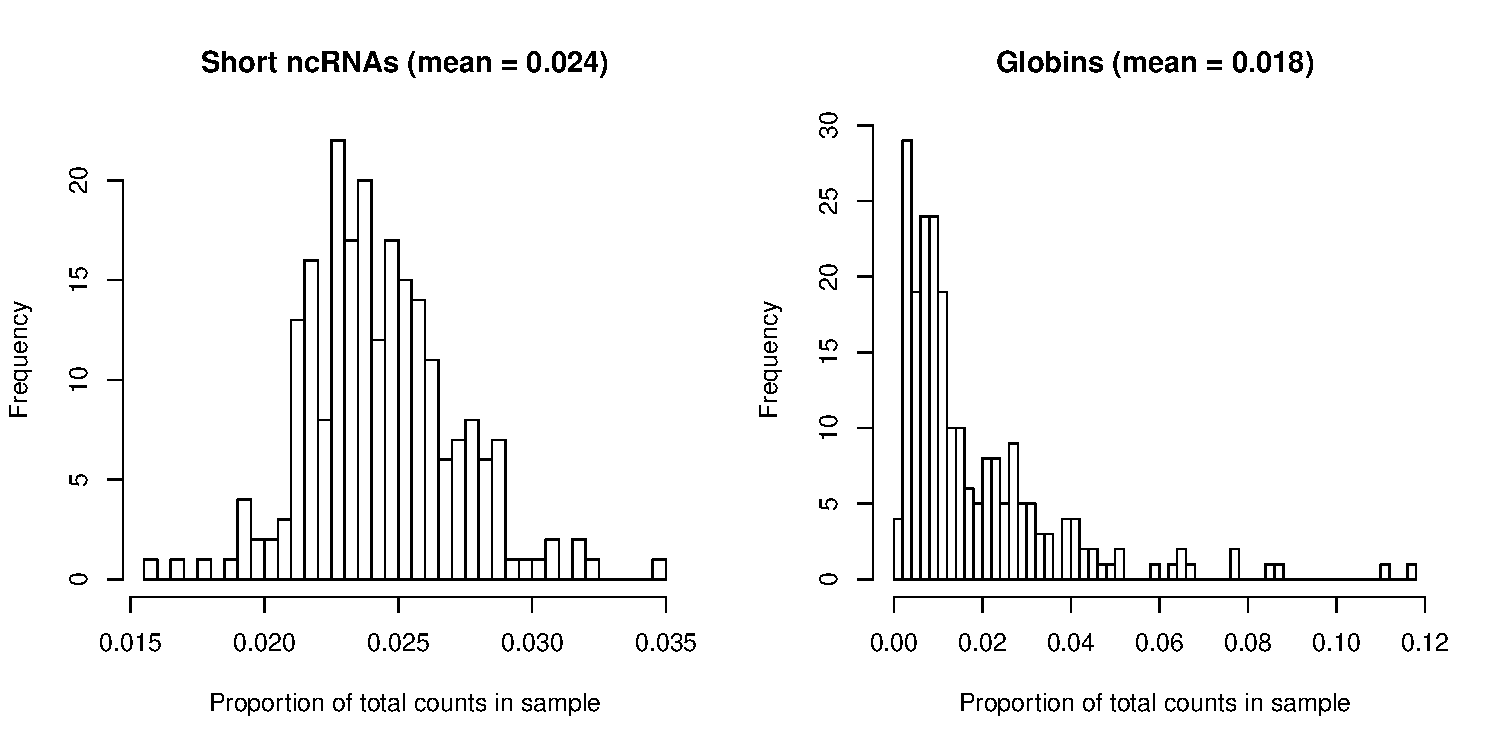
\includegraphics[width=1.0\textwidth, page=1]{mainmatter/figures/chapter_02/rnaseq_data_setup.per_sample.short_ncRNA_globin_levels_hist.pdf}
    \caption{Distributions of removed short ncRNA and globin counts as a proportion of total counts in \gls{RNAseq} samples.}
    \label{fig:hird_shortncRNA_and_globins}
\end{figure}

Many of the genes in the reference transcriptome are not expressed in \gls{PBMC} (\autoref{fig:hird_rnaseq_filtering_zeroProp}), and many genes are expressed at counts too low for statistical analysis of \gls{DGE}
Genes were further filtered to require detection (non-zero expression) in at least 95\% of samples, and a minimum of 0.5 \gls{CPM} in at least 20\% of samples.
% TODO: check number of genes hit by non-zero and write a justification
The 0.5 \gls{CPM} threshold was chosen to correspond to approximately 10 counts in the smallest library, where 10-15 counts is a rule of thumb for considering a gene to be robustly expressed\autocite{chen2016ReadsGenesPathways}.
% TODO \url{https://f1000research.com/articles/5-1408/v3}
The change in the distribution of gene expressions among samples before and after filtering shows a substantial number of low expression genes are removed (\autoref{fig:hird_rnaseq_cpm_filtering}).

\begin{figure}
    \centering
    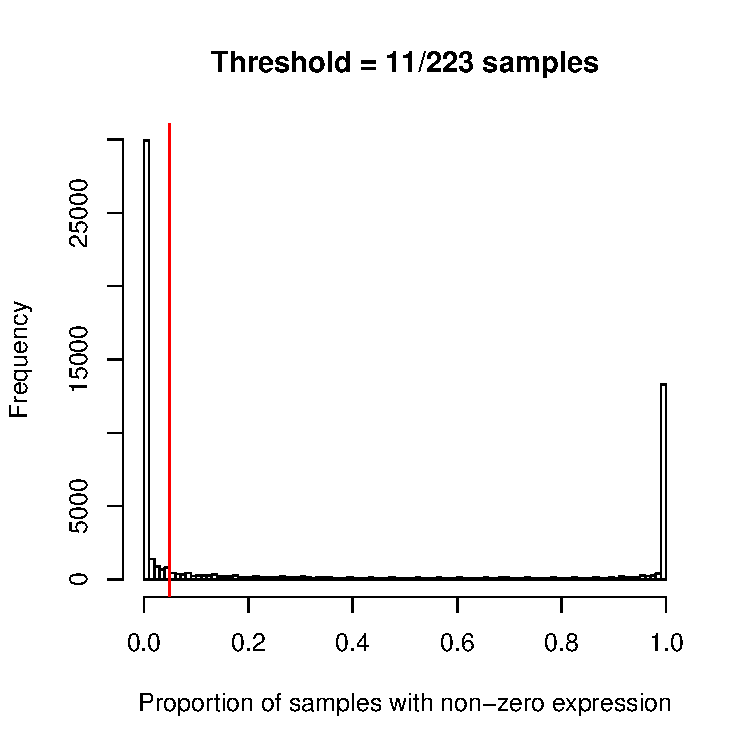
\includegraphics[width=0.6\textwidth, page=1]{mainmatter/figures/chapter_02/rnaseq_data_setup.gene_zero_prop.pdf}
    \caption{Distribution of the proportion of samples in which genes were detected (non-zero expression). Many genes are not detected in any samples. Vertical line shows 5\% threshold below which genes were discarded.}
    \label{fig:hird_rnaseq_filtering_zeroProp}
\end{figure}

\begin{figure}
    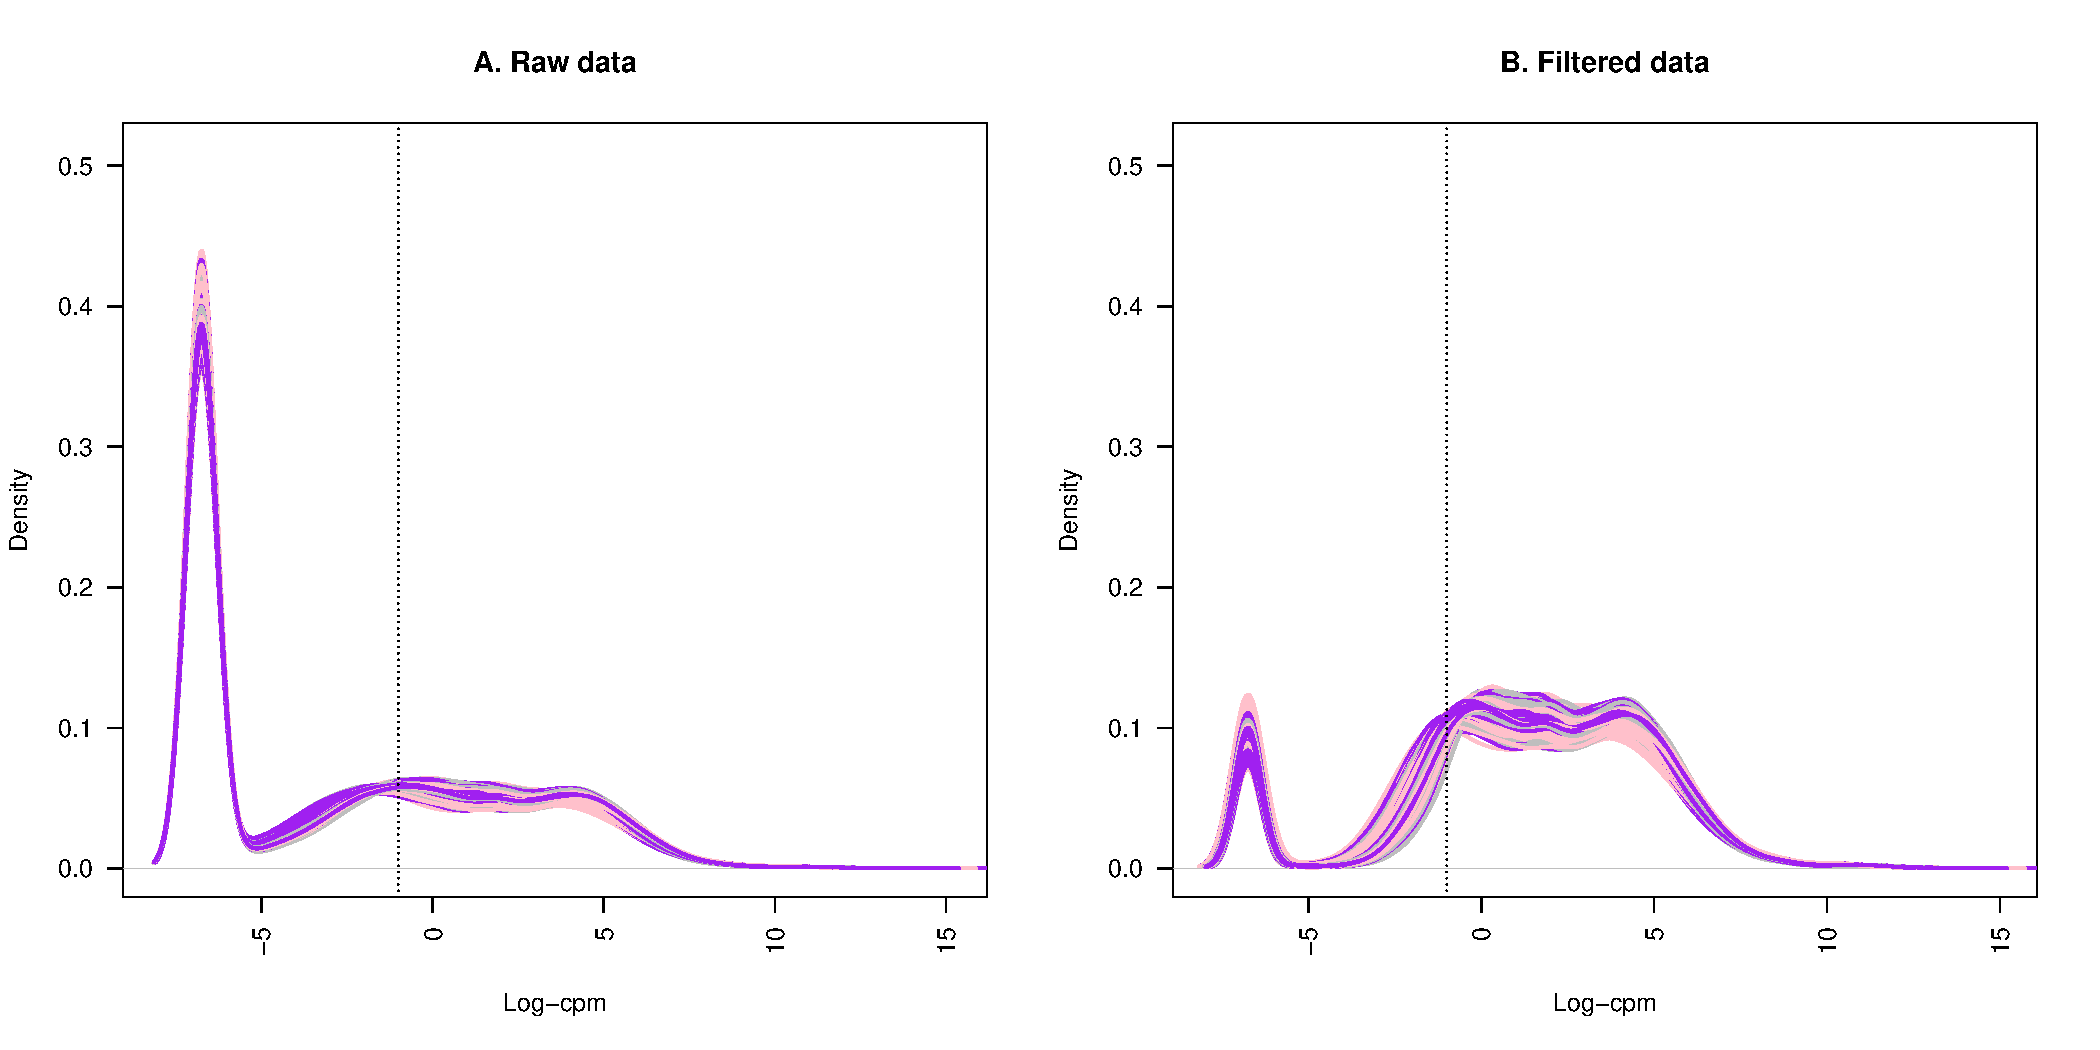
\includegraphics[width=1.0\textwidth]{mainmatter/figures/chapter_02/rnaseq_data_setup.sample_cpm_density_filtered.pdf}
    \caption{Distribution of gene expressions for \gls{RNAseq} samples before and after filtering no expression and low expression genes. Vertical line shown at \gls{CPM} = 0.5 threshold.}
    \label{fig:hird_rnaseq_cpm_filtering}
\end{figure}

After the application of all filters, expression values were available for 21626 genes over 223 samples (75/75 individuals on day 0, 73/75 on day 1, and 75/75 on day 7).

\subsection{Array data preprocessing}
\label{subsec:hird_dge_array_preproc}

% 6.	Pre-process microarray expression data
% 6.1.	Annotate Entrez and ENS ids using hgug4112a.db
% 6.1.1.	The chip is single-channel “Agilent-014850 Whole Human Genome Microarray 4x44K G4112F”
% 6.1.2.	Apparently fine to use 4112A db for 4112F https://support.bioconductor.org/p/73193/
% 6.2.	Redefine responder phenotype to be consistent with RNA-seq and Sobolev paper (>= 4-fold in HAI or MN)
% 6.3.	Background correction: limma::backgroundCorrect(x, method="normexp")
% 6.3.1.	Background comes from non-specific binding
% 6.3.2.	Pipeline from the Agi4x44PreProcess Bioconductor package (deprecated)
% 6.3.3.	Notes on Edwards: https://academic.oup.com/bioinformatics/article/23/20/2700/230165#2633725
% 6.3.3.1.	“adjusts the foreground intensities by subtracting the background when the difference between the foreground and background is larger than a small threshold value. When the difference is less than the threshold, subtraction is replaced by a smooth monotonic function.“
% 6.3.3.2.	May be preferred over normexp in our case due to “Question: Compressed boxplots after 'normexp+offset' background correction of Agilent one color microarrays in LIMMA“ https://support.bioconductor.org/p/46485/
% 6.3.3.3.	Example of Edwards used over normexp for Agilent arrays: “Modified least-variant set normalization for miRNA microarray” https://www.ncbi.nlm.nih.gov/pmc/articles/PMC2995391/
% 6.3.3.4.
% 6.3.4.	Notes on normexp:
% 6.3.4.1.	This function is designed to produce positive corrected intensities.
% 6.3.4.1.1.	“If the "normexp" method is selected, then a convolution of normal and exponential distributions is fitted to the foreground intensities using the background intensities as a covariate, and the expected signal given the observed foreground becomes the corrected intensity.”
% 6.3.4.1.2.	https://www.ncbi.nlm.nih.gov/pmc/articles/PMC2648902/ “A method normexp was introduced which models the observed intensities as the sum of exponentially distributed signals and normally distributed background values”
% 6.3.4.2.	[…] an offset value (normally 50) is used. This offset adds a constant to the intensities before log-transforming, so that the log ratios are shrunk towards zero at the lower intensities.
% 6.3.4.3.	The optimal choice for the offset is the one which makes the variability of the log-ratios as constant as possible across the range of intensity values (Smyth, G. in BioC mailing List, https://stat.ethz.ch/pipermail/bioconductor/2006-April/012554.html ).
% 6.3.5.	Choice of offset: https://academic.oup.com/nar/article/38/22/e204/1049223#93002104
% 6.3.5.1.	Adding an offset to the intensities before log transformation not only was found to lower the variance (improve precision) but also to compress the fold-change range and increase bias. In other words, offsets decrease noise but increase bias.
% 6.3.5.2.	The normexp by control (neqc) algorithm […] For routine practical use, we recommend modest offsets for Illumina data in the range of 10–50, which minimize the bias while still delivering a benefit in terms of FDR. Offsets of 16–50 have been used in a number of biological studies (10,13,16). These results remain essentially unchanged whether or not control probes are used […]  The default offset is 16, which seems generally to give good results on recent versions of human and mouse Illumina arrays.
% No need for normalizeWithinArrays in 2 color.
% 6.4.	Between-sample normalization: Limma::normalizeBetweenArrays(y, method="quantile")
% Why quantile normalise arrays? "A comparison of normalization methods for high density oligonucleotide array data based on variance and bias"
% 6.4.1.	Note that we omit any normalize within arrays procedures, as this is a single-channel array
% 6.4.2.	Normalization is the attempt to compensate for systematic technical differences between chips
% 6.4.3.	Uses https://www.rdocumentation.org/packages/limma/versions/3.28.14/topics/normalizeQuantiles
% 6.4.3.1.	“Each quantile of each column is set to the mean of that quantile across arrays. The intention is to make all the normalized columns have the same empirical distribution. This will be exactly true if there are no missing values and no ties within the columns: the normalized columns are then simply permutations of one another.”
% 6.4.4.	Also see this “StatQuest: Quantile Normalization” https://www.youtube.com/watch?v=ecjN6Xpv6SE
% 6.4.5.	This also does a log2 transform, so final units are normalized log2 intensity
%
Single-channel Agilent 4x44K microarray (G4112F) data for 173 samples from \autocite{sobolev2016AdjuvantedInfluenzaH1N1Vaccination} were downloaded from ArrayExpress\footnote{\url{https://www.ebi.ac.uk/arrayexpress/experiments/E-MTAB-2313/}}.
These arrays were originally processed in two batches, the effect of which is seen in the raw foreground intensities (\autoref{fig:hird_array_boxplots_raw}).

\begin{figure}
    \centering
    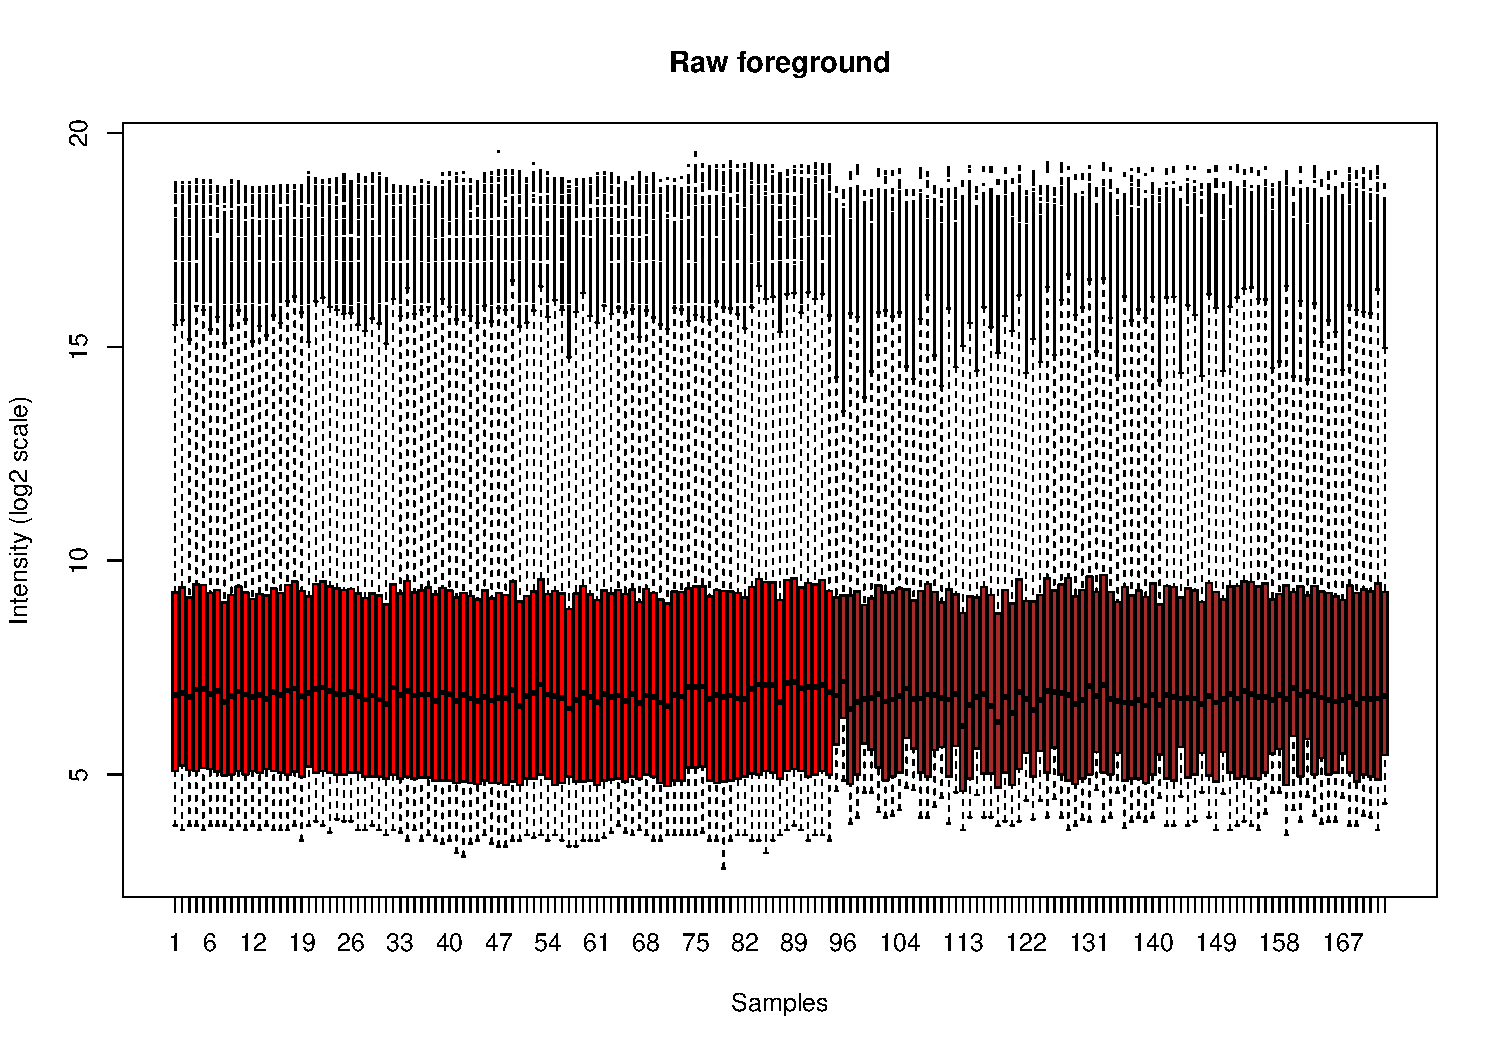
\includegraphics[width=1.0\textwidth,page=1]{mainmatter/figures/chapter_02/array_data_setup.array_intensity_boxplots.pdf}
    \caption{Raw foreground intensities for 173 \gls{HIRD} array samples. Colored by array processing batch.}
    \label{fig:hird_array_boxplots_raw}
\end{figure}

% Actually uses:
% The so-called glog2 (short for generalised logarithm) is a function that is like the logarithm (base 2) for large values (large compared to the amplitude of the background noise), but is less steep for smaller values.
VSN\autocite{huber2002VarianceStabilizationApplied} was used to perform background correction, between-array normalisation, and variance-stabilisation of intensity values, resulting in expression values on a $\log_2$ scale.

% 6.5.	Summarise probes (into loci): WGCNA::collapseRows(rowGroup=Ensembl ID, method="MaxMean", connectivityBasedCollapsing=FALSE)
% 6.5.1.	https://www.ncbi.nlm.nih.gov/pmc/articles/PMC3166942/
% 6.5.1.1.	“For example, we find that in most microarray experiments performed on brain tissue it is best to choose the probe with the maximum mean expression per gene, whereas when choosing a single gene to represent a co-expression module, the optimal collapsing method depends on the goal of the analysis.”
% 6.5.1.2.	“In the case of collapsing probes to their respective gene symbols, for example, we find that the 1.max strategy (implemented by setting method = "MaxMean" and connectivityBasedCollapsing = FALSE) produces the most robust results.”
% 6.5.1.3.	i.e. choose the probe with the highest mean of expression over the samples
Most genes are targetted by multiple array probes; 31208 probes were collapsed into 18216 Ensembl genes using by selecting the probe with the highest mean intensity for each gene (\texttt{WGCNA::collapseRows(method=MaxMean)}, recommended for probe to gene collapsing\autocite{miller2011StrategiesAggregatingGene}).
While it would be optimal to select a collapsing method to maximise the concordance between array and \gls{RNAseq} expression values, there were no samples assayed by both platforms in the \gls{HIRD} dataset.
The final normalised $\log_2$ intensity values for these 18216 genes over 173 samples is shown in \autoref{fig:hird_array_boxplots_MaxMean}.

\begin{figure}
    \centering
    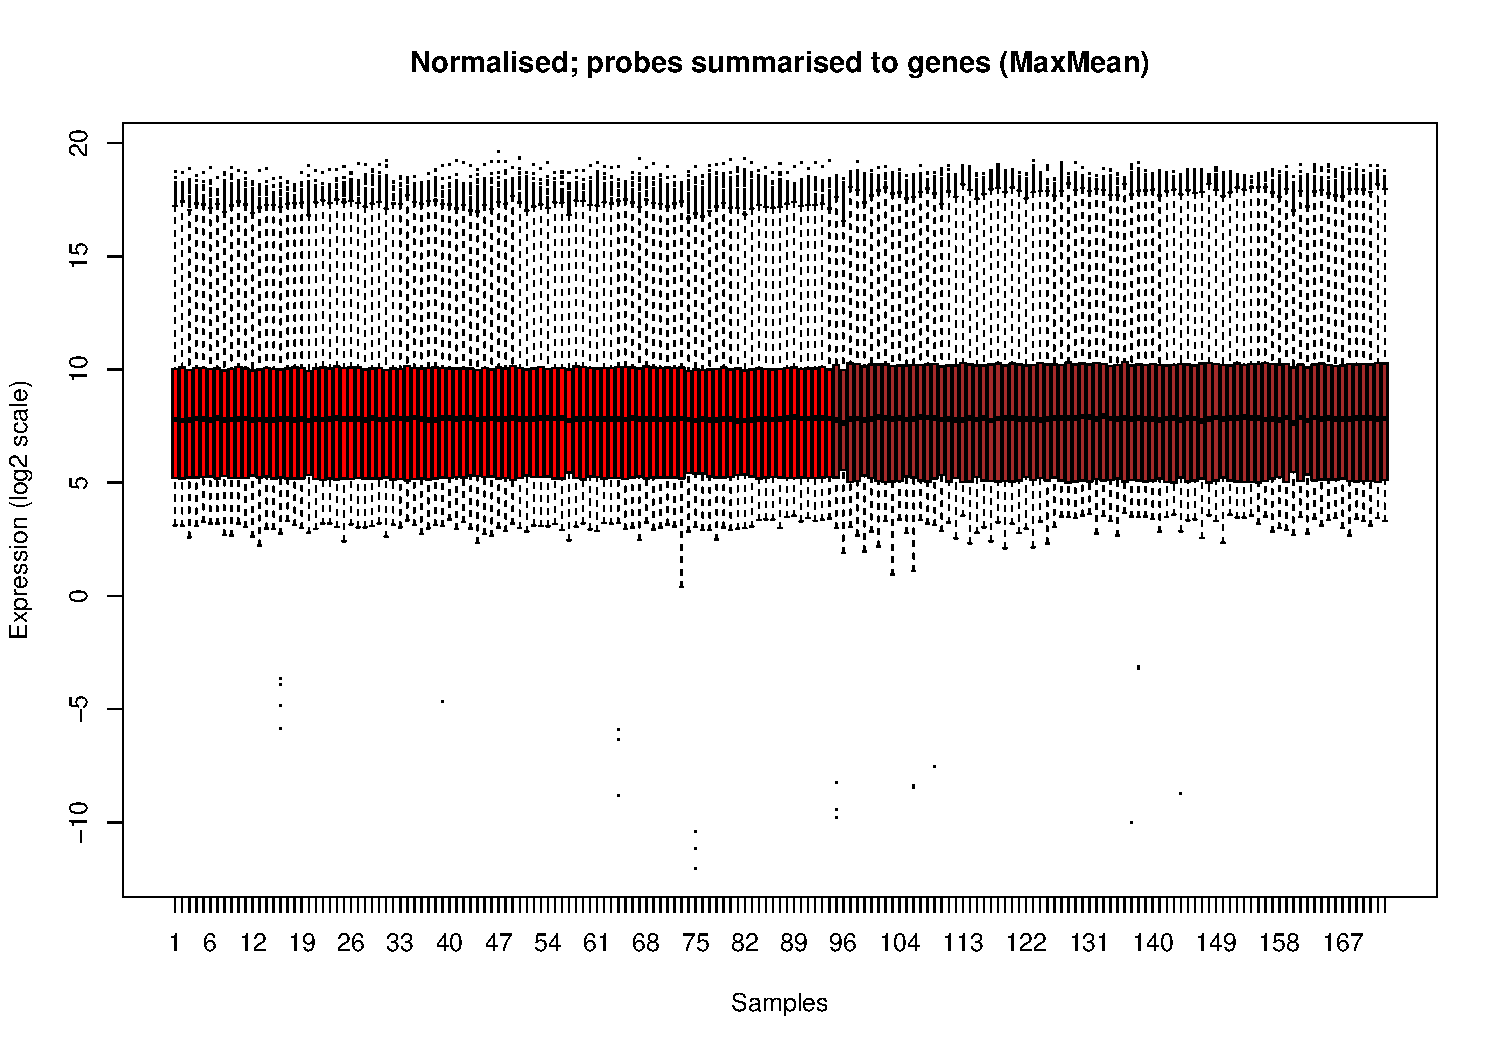
\includegraphics[width=1.0\textwidth]{mainmatter/figures/chapter_02/array_data_setup.array_intensity_boxplots.MaxMean.pdf}
    \caption{Array intensity estimates after VSN normalisation and collapsing of probes to genes. Colored by array processing batch.}
    \label{fig:hird_array_boxplots_MaxMean}
\end{figure}

\subsection{\Glsfmtlong{DGE}}

% TODO: https://github.com/matloff/regtools/blob/master/inst/ScalingInPCA.md?s=09
\gls{PCA} of the expression data reveals although samples separate by experimental timepoint along \gls{PC}3 (\autoref{fig:hird_expression_pcs}d), measurement platform is by far the largest source of variation.
% TODO: note no filtering of expression data before pca due to wanting to see batch fx
Normalisation was also not able to completely remove the batch effect within the array data (\autoref{fig:hird_expression_pcs}a).
% Also see:
% Wang, C., Gong, B., Bushel, P. R., Thierry-Mieg, J., Thierry-Mieg, D., Xu, J., Fang, H., Hong, H., Shen, J., Su, Z., Meehan, J., Li, X., Yang, L., Li, H., Łabaj, P. P., Kreil, D. P., Megherbi, D., Gaj, S., Caiment, F., … Tong, W. (2014). The concordance between RNA-seq and microarray data depends on chemical treatment and transcript abundance. Nature Biotechnology, 32(9), 926–932. https://doi.org/10.1038/nbt.3001
%
% TODO: THE rnaseq review paper: https://www.nature.com/articles/nrg2484
% Figure 2: Quantifying expression levels: RNA-Seq and microarray compared.
% The CBM paper intro has a good summary too. https://www.ncbi.nlm.nih.gov/pmc/articles/PMC5510692/
The large platform effect likely stems from systematic technological differences in how each platform measures expression.
For example, arrays suffer from ratio compression due to cross-hybridisation\autocite{draghici2006ReliabilityReproducibilityIssues}.
\gls{RNAseq} has a higher dynamic range, resulting less bias at low expression levels, but estimates are more sensitive to changes in depth than array estimates are to changes in intensity \autocite{robinson2015NestedParallelExperiment}.
There are also differences in the statistical models behind expression quantification and normalisation, as described above\todo{cite relevant preprocessing sections}.

Despite the shortcomings of array data detailed above, the array dataset tends to contain individuals with more extreme antibody response phenotypes (\autoref{fig:hird_phenotypes_by_platform}), and hence the data should not be excluded.
Given the magnitude of the platform effect, I concluded that the appropriate approach should be a two-stage approach that integrates per-platform \gls{DGE} effect estimates while explicitly accounting for between-platform heterogeneity.

\begin{figure}
    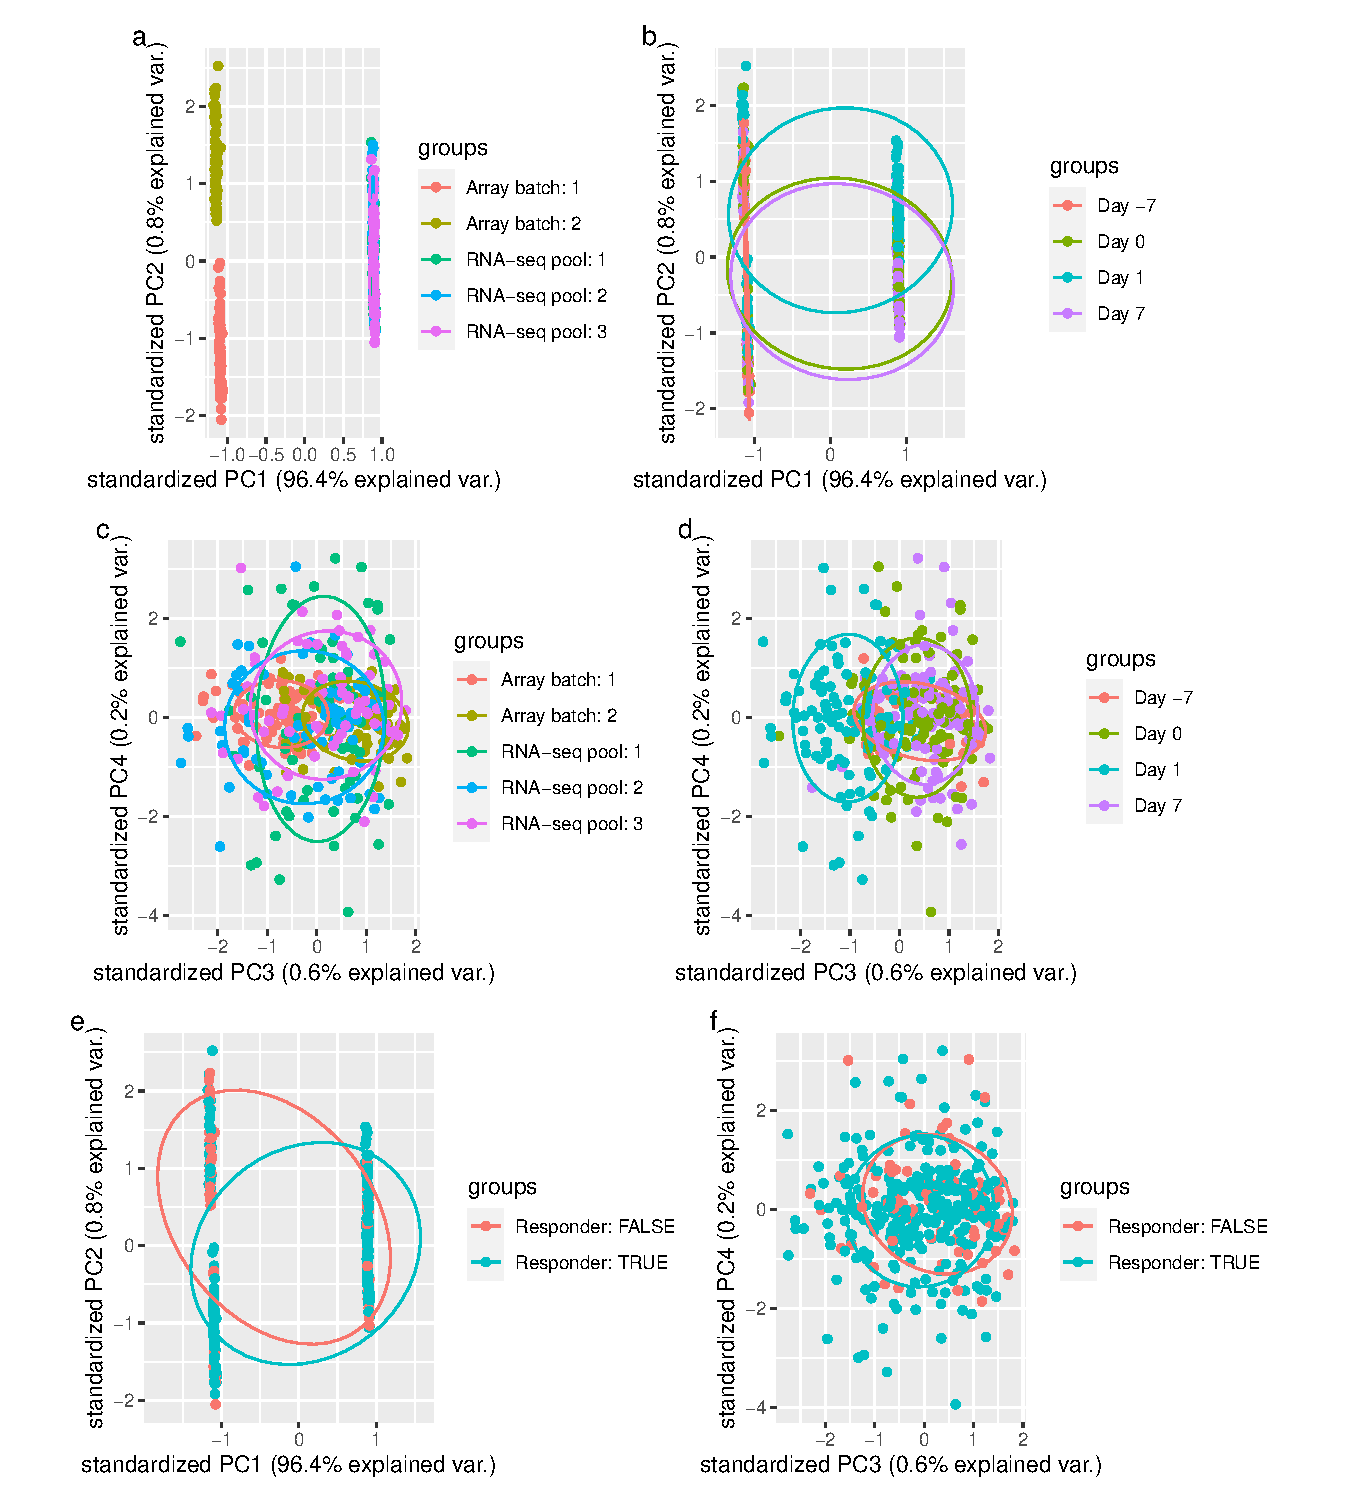
\includegraphics[width=1.0\textwidth,page=1]{mainmatter/figures/chapter_02/compare_phenotype_by_platform.E_pca.pdf}
    \caption{First four \glspl{PC} in the \gls{HIRD} expression data, colored by platform and batch (left), and timepoint (right).}
    \label{fig:hird_expression_pcs}
\end{figure}

% Also see: https://support.bioconductor.org/p/72815/
Regarding the batch effect within the array data, a popular adjustment method is ComBat\autocite{johnson2007AdjustingBatchEffects}, which estimates centering and scaling parameters by pooling information across all genes using empirical Bayes.
\todo{combat does have a pro in that it can do per gene scaling, that fixed fx won't do}
ComBat is the method used in \autocite{sobolev2016AdjuvantedInfluenzaH1N1Vaccination}.
In comparisons of microarray batch effect adjustment methods, ComBat performs favourably (vs. five other adjustment packages)\autocite{chen2011RemovingBatchEffects} or comparably (vs. batch as a fixed or random effect in the linear model)\autocite{espin-perez2018ComparisonStatisticalMethods}.
However, where batches are unbalanced in terms of sample size\autocite{zhang2018AlternativeEmpiricalBayes} or distribution of study groups that have an impact on expression\autocite{nygaard2015MethodsThatRemove}, ComBat can overcorrect batch differences or bias estimates of group differences respectively.
In our data, sample size and timepoint groups are fairly balanced between the two array batches, but the proportion of responders is not\autoref{tab:hird_batch_balance}, hence I elect not to use ComBat to pre-adjust the array expression data, and model the batches as fixed effects.
In practice, results from the \gls{DGE} analysis were not substantially affected by the choice of whether to use a ComBat pre-adjustment or a fixed effect.
\todo{this is not a very precise justification. actually, if I were to color R/NR in the PCA plot, R/NR doesn't really explain a lot of var in global gene expression. that's probably why the results don't change much.}
\todo{weaken this. combat is used multiple times in ch3}
\todo{be more specific about how combat works i.e. estimates factors per gene per batch?}

\begin{table}[] 
 \centering 
 \caption[\captionshort{Distribution of \gls{HIRD} samples among timepoint and responder groups in the array batches and \gls{RNAseq} pools.}]{\textbf{Distribution of \gls{HIRD} samples among timepoint and responder groups in the array batches and \gls{RNAseq} pools.} Values are count and percentage for categorical variables; mean and standard deviation for continuous variables.}\label{tab:hird_batch_balance}
 \begin{tabular}{ l c c c c c c }
 \toprule
  &   &  \multicolumn{ 5 }{c}{ Array batch/\gls{RNAseq} pool }\\ 
  & Total & Array 1 & Array 2 & \gls{RNAseq} 1 & \gls{RNAseq} 2 & \gls{RNAseq} 3\\ 
  & n = 374 & n = 87 & n = 79 & n = 70 & n = 69 & n = 69 \\ 
  \midrule
 Day &   &   &   &   &   &  \\ 
 \hspace{6pt}    -7 & 40 (10.7\%) & 20 (23\%) & 20 (25.3\%) & 0 (0\%) & 0 (0\%) & 0 (0\%)\\ 
 \hspace{6pt}    0 & 114 (30.5\%) & 24 (27.6\%) & 20 (25.3\%) & 24 (34.3\%) & 23 (33.3\%) & 23 (33.3\%)\\ 
 \hspace{6pt}    1 & 109 (29.1\%) & 21 (24.1\%) & 20 (25.3\%) & 22 (31.4\%) & 23 (33.3\%) & 23 (33.3\%)\\ 
 \hspace{6pt}    7 & 111 (29.7\%) & 22 (25.3\%) & 19 (24.1\%) & 24 (34.3\%) & 23 (33.3\%) & 23 (33.3\%)\\ 
 Responder &   &   &   &   &   &  \\ 
 \hspace{6pt}    FALSE & 80 (21.4\%) & 12 (13.8\%) & 36 (45.6\%) & 11 (15.7\%) & 9 (13\%) & 12 (17.4\%)\\ 
 \hspace{6pt}    TRUE & 294 (78.6\%) & 75 (86.2\%) & 43 (54.4\%) & 59 (84.3\%) & 60 (87\%) & 57 (82.6\%)\\ 
 TRI &   &   &   &   &   &  \\ 
 \hspace{6pt}   & -0.1 (1.0) & -0.1 (1.0) & -0.4 (1.4) & 0.1 (0.6) & -0.0 (0.8) & 0.2 (0.6)\\ 
 \bottomrule
 
 \end{tabular}
 \end{table}


\subsubsection{Per-platform \glsfmtlong{DGE} model}

% Also used arrayWeights as precision weight inputs to lmFit
% See: https://bmcbioinformatics.biomedcentral.com/articles/10.1186/1471-2105-7-261#Bib1
% The method successfully assigns lower weights to less reproducible arrays from different experiments. Down-weighting the observations from suspect arrays increases the power to detect differential expression.
For the array data, as \autocite{sobolev2016AdjuvantedInfluenzaH1N1Vaccination} demonstrated no significant global differences in expression between day -7 and day 0, I likewise merge these two timepoints into a single \enquote{day 0} baseline timepoint in the following \gls{DGE} models.

% 5.6.	Between-sample normalization of library size: Trimmed mean of M-values (TMM)
% Selecting between-sample RNA-Seq normalization methods from the perspective of their assumptions https://www.ncbi.nlm.nih.gov/pmc/articles/PMC6171491/
% 5.6.1.	edgeR::calcNormFactors generates norm.factors for each sample
For the \gls{RNAseq} data, between-sample normalisation factors were computed using the \gls{TMM} method\autocite{evans2018SelectingBetweensampleRNASeq} from edgeR::calcNormFactors\autocite{robinson2010EdgeRBioconductorPackage}; 
% TODO: define composition bias that TMM corrects, see evans2018SelectingBetweensampleRNASeq
% also see https://rnajournal.cshlp.org/content/early/2020/04/13/rna.074922.120.full.pdf
% TODO: Note: calcNormFactors doesn’t normalize the data, it just calculates normalization factors for use downstream.
then variance-stabilisation was performed using voom\autocite{law2014VoomPrecisionWeights}, resulting in expression values with units of $\log_2{\text{\gls{CPM}}}$.
\todo{this is DGE specific normalisation, which is why it goes here, not in the preprocessing section}
% TODO:
% voom does t(log2(t(counts + 0.5)/(lib.size + 1) * 1e+06)), where lib.size considers norm.factors, it does not variance-stabilise.
% The idea is to use precision weights for each observation instead.

% 7.	Differential expression (limma)
% 7.2.	Create contrasts
% 7.3.	Estimate within-block correlation (duplicateCorrelation), using individuals as blocks
% 7.4.	Array data only: Compute sample quality weights for each array (arrayWeightsSimple(v, design=mod1))
% 7.5.	RNA-seq data only: Correct for mean-variance trend (voom)
% 7.5.1.	http://web.mit.edu/~r/current/arch/i386_linux26/lib/R/library/limma/html/voom.html
% 7.5.1.1.	“voom is an acronym for mean-variance modelling at the observational level. The key concern is to estimate the mean-variance relationship in the data, then use this to compute appropriate weights for each observation. Count data almost show non-trivial mean-variance relationships. Raw counts show increasing variance with increasing count size, while log-counts typically show a decreasing mean-variance trend. This function estimates the mean-variance trend for log-counts, then assigns a weight to each observation based on its predicted variance. The weights are then used in the linear modelling process to adjust for heteroscedasticity.”
% 7.5.1.2.	“voom performs the following specific calculations. First, the counts are converted to logCPM values, adding 0.5 to all the counts to avoid taking the logarithm of zero. The matrix of logCPM values is then optionally normalized. The lmFit function is used to fit row-wise linear models. The lowess function is then used to fit a trend to the square-root-standard-deviations as a function of average logCPM. The trend line is then used to predict the variance of each logCPM value as a function of its fitted value, and the inverse variances become the estimated precision weights.”
% 7.6.	(lmFit)
% 7.7.	(contrasts.fit)
% 7.8.	(eBayes/treat)
% 7.8.1.1.1.	https://rdrr.io/bioc/limma/man/ebayes.html
% 7.8.1.1.1.1.	When lfc=0, treat is identical to eBayes, except that F-statistics and B-statistics are not computed.
% 7.8.1.1.2.	https://academic.oup.com/bioinformatics/article/25/6/765/251641 The TREAT fold-change threshold should be set to a low value below which no fold-change is likely to be of genuine interest. Researchers should be mindful that genes will need to exceed this threshold by some way, depending on the data, before being declared statistically significant. Our experience suggests a minimal value, such as a 10% fold-change, corresponding to τ=log2(1.1)=0.13 on the log2-scale. It would be better to interpret the threshold as ‘the fold-change below which we are definitely not interested in the gene’ rather than ‘the fold-change above which we are interested in the gene’.
% 7.9.	(decideTests)
Linear models were fit using limma\autocite{ritchie2015LimmaPowersDifferential}, which is computationally fast, and performs well for sufficiently large ($n \ge 3$ per group) sample sizes\autocite{soneson2013ComparisonMethodsDifferential}.
For each gene, I fit a model (model 1) with expression as the response variable; with timepoint (baseline, day 1, day 7), \gls{TRI}, batch, sex, age, and the first 4 genotype \glspl{PC} as fixed-effect predictors; and individual as a random-effect predictor.
% TODO: age is assumed linear here
\todo{link to papers justifying sex, age, ancestry as significant effects on immune gene expression}
\todo{add equation from ch3. especially justify having TRI in as predictor, by noting equiv of traditional lm to contrasts}
% TODO: The peril of adjusting for baseline when using change as a predictor
% https://bioconductor.org/packages/release/bioc/vignettes/variancePartition/inst/doc/dream.html
% Limma has a built-in approach for analyzing repeated measures data using duplicateCorrelation(). The model can handle a single random effect, and forces the magnitude of the random effect to be the same across all genes.
% ...
% The duplicateCorrelation method estimates a single variance term genome-wide even though the donor contribution of a particular gene can vary substantially from the genome-wide trend.
Within-individual correlations for the random effect were estimated using limma::duplicateCorrelation.
A second model (model 2) was also fit, including 3 additional terms for the interactions between each timepoint and \gls{TRI}.
%
% See: https://stats.stackexchange.com/questions/151730/test-if-two-coefficients-are-statistically-different-in-logistic-regression
Contrasts were defined, testing if linear combinations of estimated coefficients are different from zero.
% TODO: What is a contrast? A contrast is essentially a difference in regression coefficients. We have seen that the regression coefficients can express a difference in means or a single mean, as well as the slope and intercept of a line. A contrast is a way of testing more general hypotheses about population means.
% A contrast is defined as the sum of each group mean multiplied by a coefficient for each group
% In statistics, particularly in analysis of variance and linear regression, a contrast is a linear combination of variables (parameters or statistics) whose coefficients add up to zero, allowing comparison of different treatments.[1][2]
From model 1, I defined contrasts for day 1 vs. baseline, day 7 vs. baseline, day 7 vs. day 1, \gls{TRI}, sex, and age.
% TODO
% The grand mean or pooled mean is the mean of the means of several subsamples, as long as the subsamples have the same number of data points.
% \2 NOTE: this is not the same as the same as the mean of means contrast as pooled is not mean of two means
From model 2, I defined contrasts for the \gls{TRI} specifically at each of the three timepoints.
% TODO: by merely specifying the model with interactions, we allow them, and thus change the interp. thus both required
% TODO: did i really define contrasts? put in actual model equation here
%
% https://support.bioconductor.org/p/70175/
% es <- fit2$coefficients
% es_se <- sqrt(fit2$s2.post) * fit2$stdev.unscaled
Corresponding coefficients and standard errors for the contrasts were extracted from the linear models, which represent effect size in units of $\log_2$ expression fold change per unit change in predictor value.

\subsubsection{Choice of \glsfmtlong{DGE} meta-analysis method}
\label{subsubsec:hird_dge_meta_methodChoice}

In the section \todo{add section labels}, I concluded that a two-stage meta-analysis approach would be appropriate.
This meta-analysis is restricted to 13593 genes assayed by both the array and \gls{RNAseq} platforms.
% While there is abundant literature on single-plaform (e.g. \autocite{tseng2012ComprehensiveLiteratureReview}) methods [...]
%
% Examples from literature
%
% random effects:
%
% https://academic.oup.com/nar/article/45/17/9860/4084660#106485896
% - for example of REM of 24 array datasets
%
% Sweeney, T. E., Haynes, W. A., Vallania, F., Ioannidis, J. P., & Khatri, P. (2017). Methods to increase reproducibility in differential gene expression via meta-analysis. Nucleic Acids Research, 45(1), e1–e1. https://doi.org/10.1093/nar/gkw797
% - DGE random effects models should be possible with around 6-7 studies.
%
% SVA:
% Comparative RNA-Seq and Microarray Analysis of Gene Expression Changes in B-Cell Lymphomas of Canis familiaris
% https://www.ncbi.nlm.nih.gov/pmc/articles/PMC3617154/
% - applying SVA to our data revealed a strong correlation with known technical biases associated with RNA-Seq [26]–[28], [51] and removing the associated variation from the RNA-Seq samples resulted in the two technologies pairing by individual sample.
% - First, we have not attempted to capture differences in dynamic range between RNA-Seq and microarray. It is reasonable to expect that the larger dynamic range of RNA-Seq will result in larger variation. We found latent variation to be highly associated with GC content but, in contrast, found no clear evidence of an association pointing to nonlinear response in the microarrays. Second, the model underlying SVA does not explicitly capture different latent variables for the different technologies.
%
% MetaVolcano:
% The MetaVolcanoR R package combines differential gene expression results. It implements three strategies to summarize gene expression activities from different studies. i) Random Effects Model (REM) approach. ii) a vote-counting approach, and iii) a p-value combining-approach.
% - doesn't solve our small k problem
%
% CorMotif:
% https://academic.oup.com/biostatistics/article/16/1/31/259492
% - In contrast, a model that naively enumerates and analyzes all possible differential patterns across studies can deal with study-specificity and allow information pooling, but the complexity of its parameter space grows exponentially as the number of studies increases.
% - Here, we propose a correlation motif approach to address this dilemma. This approach searches for a small number of latent probability vectors called correlation motifs to capture the major correlation patterns among multiple studies.
% - First applies limma (Smyth, 2004) to each study separately. CorMotif is made for microarray data since it was motivated by the microarray analysis in the Sleep for Health in Hospital Programme (SHH) study. However, the idea behind CorMotif is general, and it should be straightforward to develop a similar framework for RNA-seq data.
% - designed for large k, seems similar to mashr
%
% CBM (“Cross-platform Bayesian Model”):
% - In this article, we propose a Bayesian hierarchical model to jointly integrate microarray and RNA-seq studies.
% - Since systematic fold change differences across RNA-seq and microarray for detecting differentially expressed genes have been previously reported, we replicated this finding in several real datasets and showed that incorporation of a normalization procedure to account for the bias improves the detection accuracy and power.
% - Cannot acually use CBM, as it operates on expressions, with a binary case vs control, so no covariates
%
% RankProd:
% - The Bioconductor package RankProd provides a new and intuitive tool for this purpose in detecting differentially expressed genes under two experimental conditions.
%
% Mayday seasight:
% - Uses a rank product model internally

Two popular frameworks for effect size meta-analysis are fixed-effect and random-effects\autocite{cohn2003HowMetaanalysisIncreases,borenstein2010BasicIntroductionFixedeffect}.
Given k studies, the fixed-effect model assumes a common population effect size shared across all studies, with observed variation explained only by sampling error.
The random-effects model assumes the k study-specific effect sizes are drawn from some distribution with variance $\tau^2$ (\gls{SD} $\tau$), representing an additional source of variation termed the between-studies heterogeneity, reducing to the fixed-effect model when $\tau=0$.
In the \gls{HIRD} data, there are $k=2$ 'studies' (array and \gls{RNAseq}), where the platform differences described in section\todo{add label} contribute to considerable between-studies heterogeneity.
The assumption of $\tau=0$ is unrealistic, hence a random-effects model is more appropriate.
\todo{make all the notation in this section consistent with, and add the equation 2.1. The normal-normal hierarchical model, \autocite{rover2017BayesianRandomeffectsMetaanalysis}}

Unfortunately, there is no optimal solution for directly estimating $\tau$ in random-effects meta-analyses with small k\autocite{bender2018MethodsEvidenceSynthesis}, in the case of $k=2$ especially\autocite{gonnermann2015NoSolutionCombining}.
Many estimators are available\autocite{veroniki2016MethodsEstimateBetweenstudy}, but lack of information with small k causes estimation to be imprecise, and often results in boundary values of $\tau = 0$ that are incompatible with the assumed positive heterogeneity\autocite{chung2013NondegeneratePenalizedLikelihood,friede2017MetaanalysisFewSmall}.
In such circumstances, the most sensible choice may be to incorporate prior information about model hyperparameters in a Bayesian random-effects framework\autocite{chung2013NondegeneratePenalizedLikelihood,veroniki2016MethodsEstimateBetweenstudy,friede2017MetaanalysisFewSmall,seide2019LikelihoodbasedRandomeffectsMetaanalysis}.
For this study, I use the implementation in bayesmeta \autocite{rover2017BayesianRandomeffectsMetaanalysis}, which requires priors for both effect size and between-studies heterogeneity.

\subsubsection{Prior for between-studies heterogeneity}

The choice of prior for between-studies heterogeneity is influential when k is small\autocite{seide2019LikelihoodbasedRandomeffectsMetaanalysis}.
\textcite{gelman2006PriorDistributionsVariance} considers the case of $k=3$, showing that a flat prior places too much weight on implausibly large estimates of $\tau$, and recommends a weakly informative prior that acts to regularise the posterior distribution.
% Gelman 
% - weak as in deliberately weaker than known knowledge, just serves to constrain
% - cauchy for the gentle slope in tails
% - also warns against inverse-gamma(e, e), as it can influence the posterior mean; it is not at all non-informative.
%
% Similarly, \autocite{friede2017MetaanalysisFewSmall} consider half-normals.
%
% More recent recommendations:
% \footnote{Documentation for Stan: \url{https://github.com/stan-dev/stan/wiki/Prior-Choice-Recommendations}.}
% - Gelman 2006 recommendations can actually be too weak for scale
% - Recommends Chung gamma(2, 1/A)
% - With full Bayes the boundary shouldn't be a problem (as long as you have any proper prior).
% - But with modal estimation, the estimate can be on the boundary, which can create problems in posterior predictions. For example, consider a varying-intercept varying-slope multilevel model which has an intercept and slope for each group. Suppose you fit marginal maximum likelihood and get a modal estimate of 1 for the group-level correlation. Then in your predictions the intercept and slope will be perfectly correlated, which in general will be unrealistic.
% Chung, Y., Rabe-Hesketh, S., Dorie, V., Gelman, A., & Liu, J. (2013). A Nondegenerate Penalized Likelihood Estimator for Variance Parameters in Multilevel Models. Psychometrika, 78(4), 685–709. https://doi.org/10.1007/s11336-013-9328-2
Since I assumed zero estimates for $\tau$ are unrealistic, I use a weakly-informative gamma prior recommended by \autocite{chung2013NondegeneratePenalizedLikelihood}, which has zero density at $\tau = 0$, increasing gently as $\tau$ increases.
% TODO: the key point is to not constrain the value of tau to be a single estimate from 2 data points, but assume that other genes may be informative of plausible values
This constrains $\tau$ to be positive, but still permits estimates close to zero if the data support it.
This is in constrast to priors used in other studies from the log-normal (e.g. \autocite{pullenayegum2011InformedReferencePrior,turner2015PredictiveDistributionsBetweenstudy}) or inverse-gamma (e.g. \autocite{higgins1996BorrowingStrengthExternal}) families that have derivatives or zero close to zero, thus ruling out small values of $\tau$ no matter what the data suggest; and in contrast to half-t family priors (e.g. \autocite{gelman2006PriorDistributionsVariance,seide2019LikelihoodbasedRandomeffectsMetaanalysis}), which have their mode at zero, and do not rule out $\tau=0$.

% rma.uni function
% By default, the starting value is set equal to the value of the Hedges (HE) estimator and the algorithm terminates when the change in the estimated value of \tau2 is smaller than 10^-5 from one iteration to the next.
To estimate the appropriate shape and scale parameters for the gamma empirically, a frequentist random-effects model using the \gls{REML} estimator for $\tau$ (recommended for continuous effects\autocite{veroniki2016MethodsEstimateBetweenstudy}) was first for each gene using \texttt{metafor::rma}.
Genes with small estimates of $\tau < 0.01$ were excluded, and a gamma distribution was fit to the remaining estimates using \texttt{fitdistrplus}.

\subsubsection{Prior for effect size}

While the choice of prior on $\tau$ is influential when k is small, there is usually enough data to estimate the effect size $\mu$ such that any reasonable non-informative prior can be used \autocite{gelman2006PriorDistributionsVariance,friede2017MetaanalysisFewSmall}.
\todo{why is this? is it having well powered studies? gelman is vague}
\texttt{bayesmeta} implements both flat and normal priors for $\mu$.
%
% https://github.com/stan-dev/stan/wiki/Prior-Choice-Recommendations
% For example, it is common to expect realistic effect sizes to be of order of magnitude 0.1 on a standardized scale (for example, an educational innovation that might improve test scores by 0.1 standard deviations). In that case, a prior of N(0,1) could be considered very strong, in that it puts most of its mass on parameter values that are unrealistically large in absolute value. When we say this prior is "weakly informative," what we mean is that, if there's a reasonably large amount of data, the likelihood will dominate, and the prior will not be important. If the data are weak, though, this "weakly informative prior" will strongly influence the posterior inference. The phrase "weakly informative" is implicitly in comparison to a default flat prior.
% Weakly informative prior should contain enough information to regularize: the idea is that the prior rules out unreasonable parameter values but is not so strong as to rule out values that might make sense
% Weakly informative rather than fully informative: the idea is that the loss in precision by making the prior a bit too weak (compared to the true population distribution of parameters or the current expert state of knowledge) is less serious than the gain in robustness by including parts of parameter space that might be relevant. It's been hard for us to formalize this idea.
% One principle: write down what you think the prior should be, then spread it out. The idea is that the cost of setting the prior too narrow is more severe than the cost of setting it too wide. I've been having trouble formalizing this idea.
% Don't use uniform priors, or hard constraints more generally, unless the bounds
% represent true constraints (such as scale parameters being restricted to be
% positive, or correlations restricted to being between -1 and 1).
Assuming that most genes are not differentially expressed with effect sizes distributed randomly around zero, I selected a normal prior with $N(\mu=0, \sigma^2)$, over a flat prior. As in the section above, to determine an appropriate scale, a normal distribution with mean $\mu = 0$ was fit to the distribution of effect sizes from the gene-wise frequentist models to empirically estimate $\sigma$.

% Another Cauchy example:
% Gelman, A., Jakulin, A., Pittau, M. G., & Su, Y.-S. (2008). A weakly informative default prior distribution for logistic and other regression models. The Annals of Applied Statistics, 2(4), 1360–1383. https://doi.org/10.1214/08-AOAS191
% - Cauchy 2.5
Heavy-tailed Cauchy priors have been proposed for effect size distributions in \gls{DGE} experiments to avoid over-shrinkage of true large effects in the tails\autocite{zhu2019HeavytailedPriorDistributions}.
Since \texttt{bayesmeta} does not implement a Cauchy prior, to avoid over-shrinkage, I flatten the normal prior considerably by scaling up the variance to $N(0, 100\sigma^2)$.
This is equivalent to assuming placing a 95\% prior probability that effects are less extreme than approximately $20\sigma$.\todo{the derivation here is qnorm(0.975, mean=0, sd=1*10) = 1*19.59964, bit iffy, double check this is correct}

\subsubsection{Evaluation of priors}

An example of the empirically estimated hyperparameters for the priors for the day 1 vs. baseline contrast are shown in \autoref{fig:hird_dgeMeta_priors_tau} (for $\tau$) and \autoref{fig:hird_dgeMeta_priors_mu} (for $\mu$).
For $\tau$, the final prior used was $\text{Gamma}(\text{shape}=1.5693, \text{scale}=0.0641)$.
This is comparable to \autocite{chung2013NondegeneratePenalizedLikelihood}'s default recommendation of a $\text{Gamma}(\text{shape}=2, \text{scale}=\lambda)$ prior where $\lambda$ is small.
\todo{could also include a table of all sets of parameters here?}
For $\mu$, the final prior used was $N(0, (0.3240*10)^2)$.
The tails of the non-scaled normal fit (black) are light compared to the Cauchy fit (red), which may lead to over-shrinkage, especially since there are many genes with high positive fold changes for the day 1 vs. baseline effect.

\begin{figure}
    \includegraphics[width=1.0\textwidth,page=2]{mainmatter/figures/chapter_02/meta.bayesmeta.priors.coefName_d1.vs.d0.pdf}
    \caption{Gamma prior for $\tau$ used for \texttt{bayesmeta} (blue), compared to the empirical distribution of per-gene frequentist \texttt{metafor::rma} estimates for $\tau$, for the day 1 vs. baseline effect (small estimates of $\tau < 0.01$ excluded). Empirical log-normal fit also shown (red).}
    \label{fig:hird_dgeMeta_priors_tau}
\end{figure}

\begin{figure}
    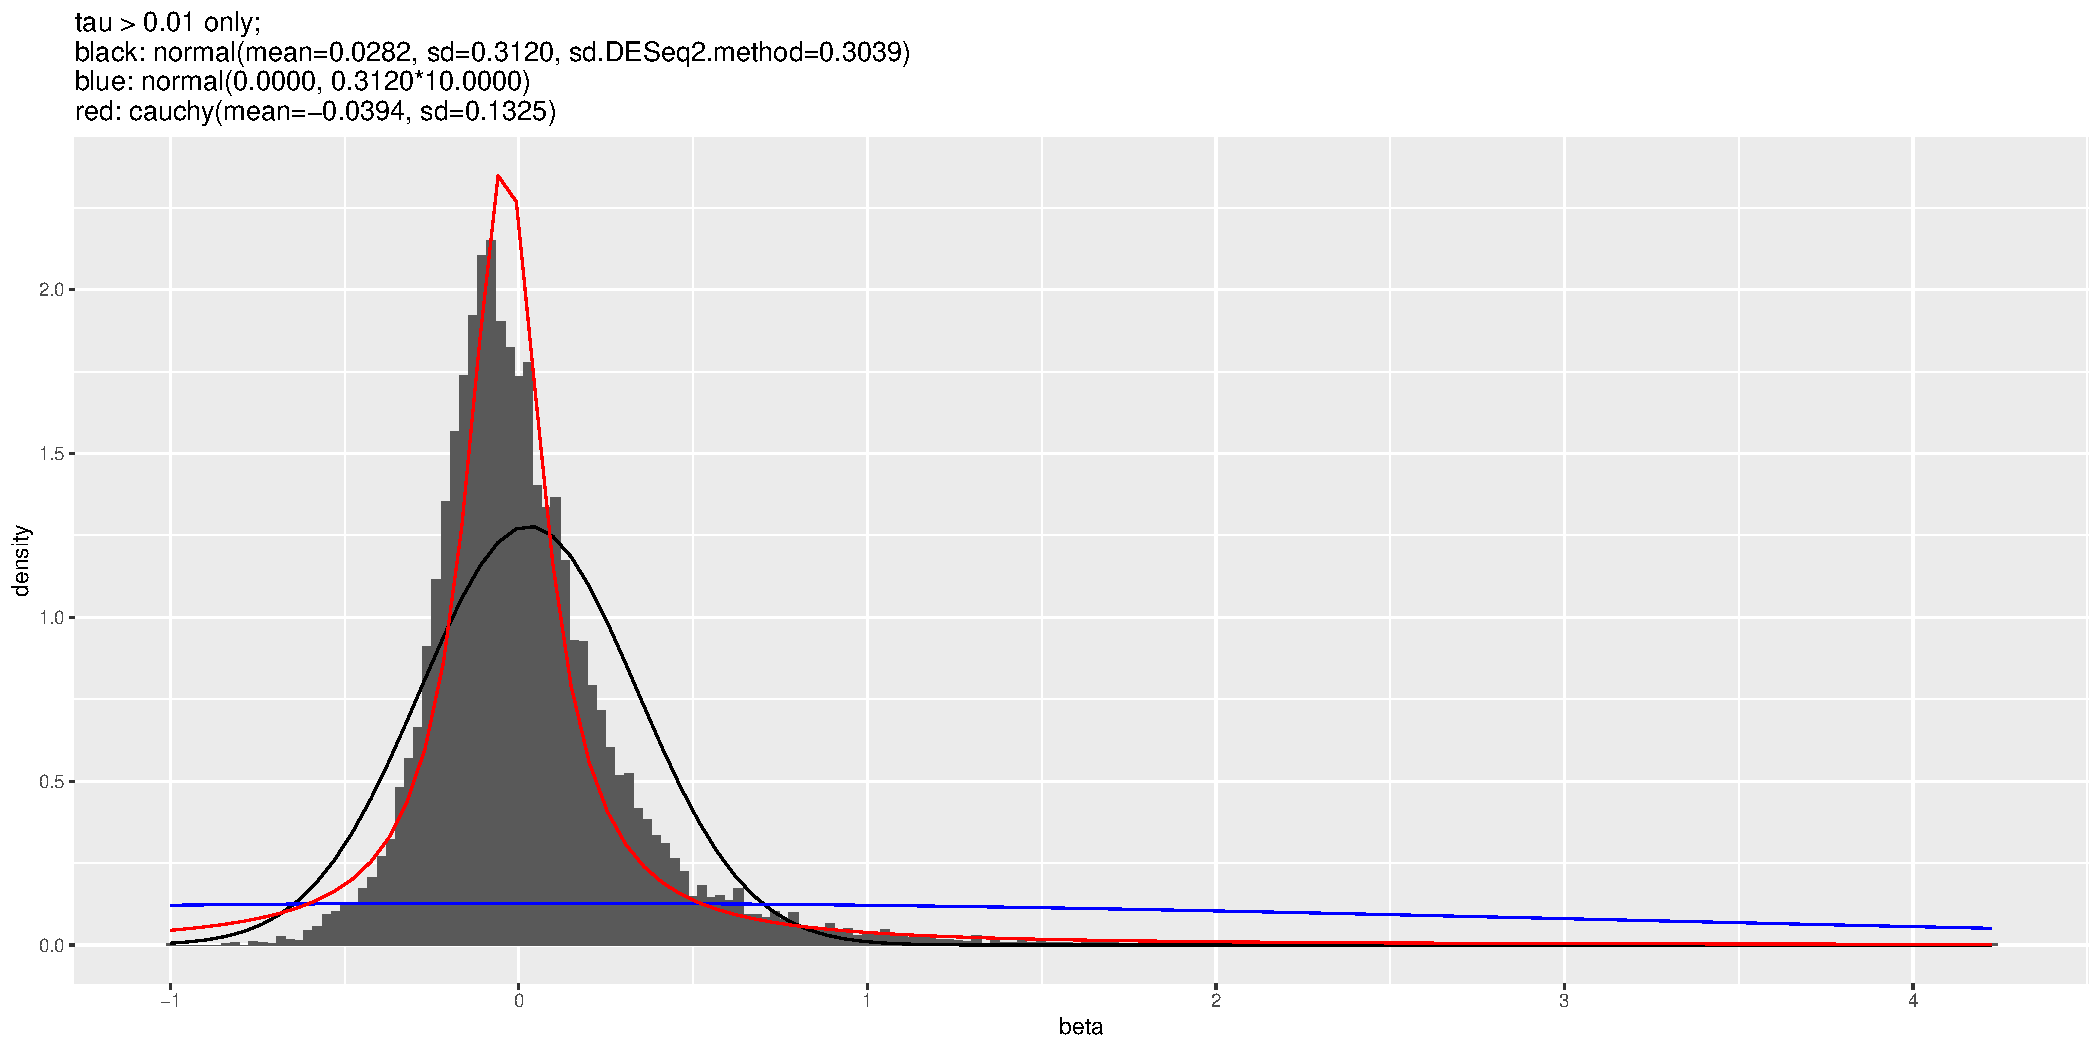
\includegraphics[width=1.0\textwidth,page=1]{mainmatter/figures/chapter_02/meta.bayesmeta.priors.coefName_d1.vs.d0.pdf}
    \caption{Normal prior for $\mu$ used for \texttt{bayesmeta} (blue), compared to the empirical distribution of per-gene frequentist \texttt{metafor::rma} estimates for $\tau$, for the day 1 vs. baseline effect. The non-scaled normal fit is shown (black), as well as a Cauchy fit (red).}
    \label{fig:hird_dgeMeta_priors_mu}
\end{figure}

\subsubsection{Multiple testing correction}

For the frequentist random-effects meta-analysis, nominal gene-wise \pvalues{} are converted to \gls{FDR} estimates using the \gls{BH} procedure (\texttt{p.adjust} in R).
% https://stats.stackexchange.com/questions/111756/the-meaning-of-positive-dependency-as-a-condition-to-use-the-usual-method-for
\todo{add note on ositive regression dependency \autocite{goeman2014MultipleHypothesisTesting}}
For the Bayesian random-effects meta-analysis, posterior effect sizes and standard errors are supplied to \texttt{ashr}, which estimates the \glspl{lfsr}, which are analogous to \gls{FDR}, but quantifies the probability of calling the wrong sign for an effect rather than than the confidence of a non-zero effect\autocite{stephens2016FalseDiscoveryRates}.
\todo{add comment on symmetry}
%
% bayesmeta
% Posterior predictive checks are implemented in the pppvalue() to generate pvalues by MCMC.
% Do not confuse with ma05$pposterior(mu=0), which is evaluation of the posterior distribution at a particular value.

\subsection{Gene set enrichment analysis using \glsfmtlongpl{BTM}}

Gene set enrichment analyses were conducted using \texttt{tmod::tmodCERNOtest}\autocite{weiner3rd2016TmodPackageGeneral}, which assesses the enrichment of small ranks within specific sets of genes compared to all genes, when the genes are ranked by some metric---here I used effect sizes from \texttt{bayesmeta}.
% TODO: alternative
% The ordering of the genes according to a certain metric is the fundament for gene enrichment analysis. tmodLimmaTest allows three orderings: p-values, "MSD" and log fold changes. The default MSD ("minimal significant difference") is the lower boundary of the 95confidence interval for positive log fold changes, and 0 minus the upper boundary of the 95better than ordering by p-value or by log fold change. See discussion in the package vignette.
%
% or TREAT from limma, or equiv testing

% FDR
% A data frame with module names, additional statistic (e.g. enrichment or AUC, depending on the test), P value and FDR q-value (P value corrected for multiple testing using the p.adjust function and Benjamini-Hochberg correction.

 % TODO: write up method for data mining, write up how redundant similarly named modules are

The gene sets used were \glspl{BTM} from\autocite{li2013MolecularSignaturesAntibody}, which are annotated sets of coexpressed genes mined from publicly available human blood transcriptomic data, and provide sets tailored for enrichment analyses in blood cells.
% TODO: why use cerno https://academic.oup.com/bioinformatics/article/35/24/5146/5511403
% TODO: which ranking metric: https://bmcbioinformatics.biomedcentral.com/articles/10.1186/s12859-017-1674-0

% TODO: add math, and comment on how CAMERA addresses assumption of correlations

\section{Results}
\todo{more text}

\subsection{Extensive global changes in expression after vaccination}

To gain an overview of how the transcriptome changes after vaccination, linear models were fit to identify genes differentially expressed at day 1 or day 7 compared to baseline (day -7 and day 0) in the \gls{HIRD} array and \gls{RNAseq} expression data, accounting for covariates such as batch effects, sex, age, \gls{TRI}, and ancestry.
At 13593 genes with expression measured by both platforms, models were fit within each platform, then effect sizes were combined using Bayesian random-effects meta-analysis.

At a $\text{\gls{lfsr}} < 0.05$ and absolute $\text{\gls{FC}} > 1.5$ cutoff, 857/13593 genes were differentially expressed between any pair of timepoints, with their expression clustering into three main clusters (\autoref{fig:hird_dge_heatmap}).
% 692 genes with high expression at day 1, 94 genes with high expression at day 7, and 59 genes with low expression at day 1
 
\begin{figure}
    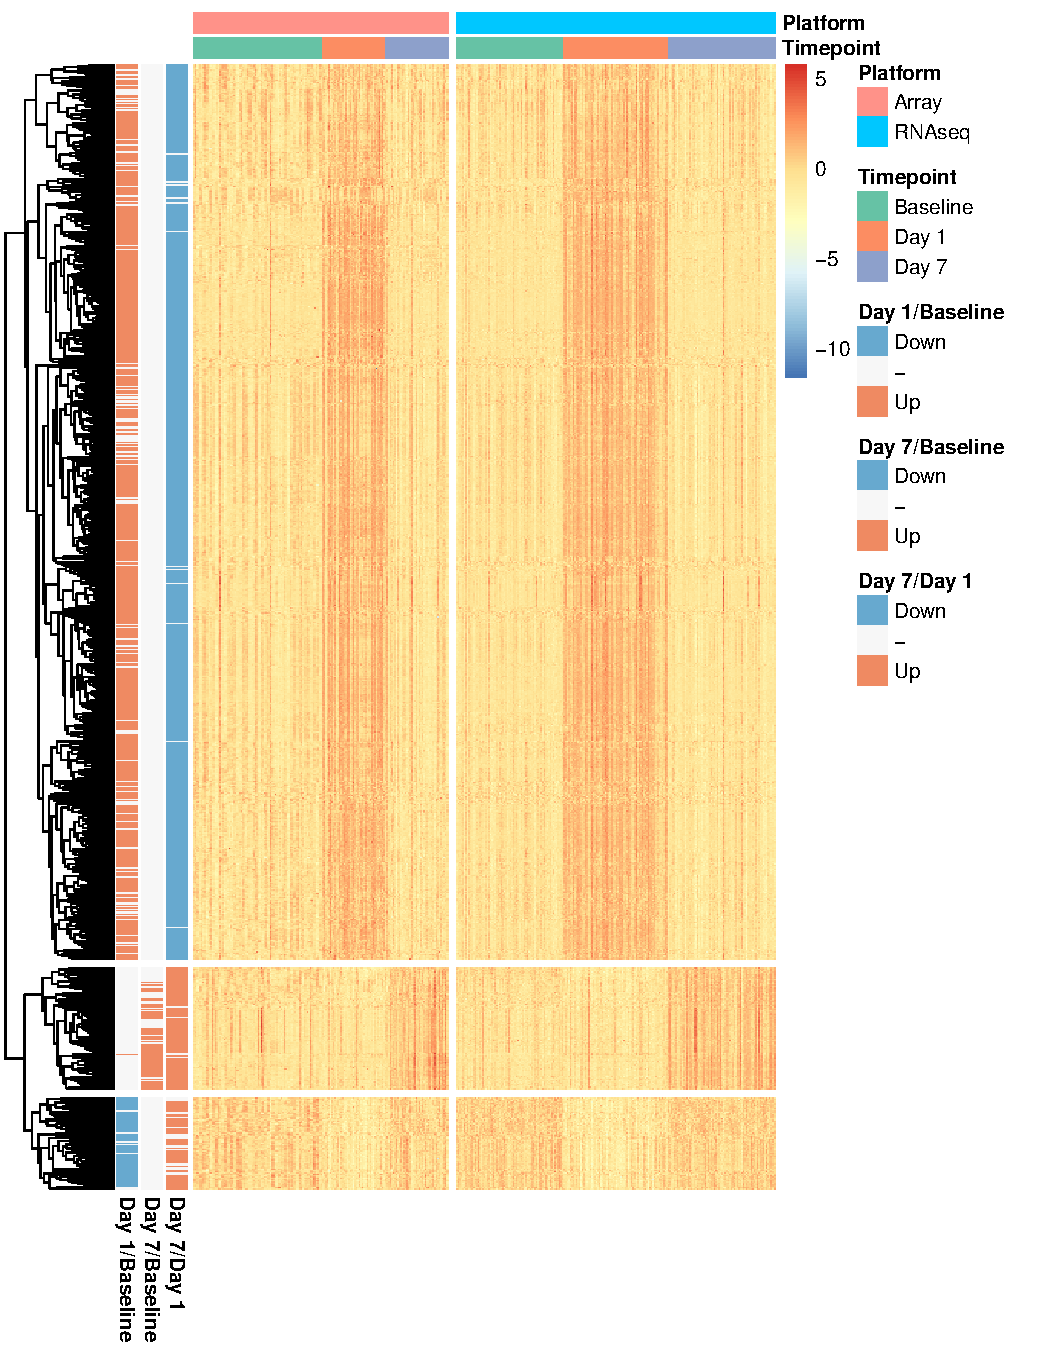
\includegraphics[width=1.0\textwidth]{mainmatter/figures/chapter_02/plot_dge_eqtl.heatmap_dge.pdf}
    \caption{Normalised gene expression for genes differentially expressed between any pair of timepoints ($\text{lfsr} < 0.05$, $\text{absolute fold change} > 1.5$) across \gls{HIRD} samples, clustered by gene (Manhattan distance metric).}
    \label{fig:hird_dge_heatmap}
\end{figure}

\subsection{Innate immune response at day 1 post-vaccination}

Consistent with global expression at day 1 being markedly different from expression at other timepoints (\autoref{fig:hird_expression_pcs}), the highest numbers of differentially expressed genes are observed at day 1, with 644 genes differentially expressed vs. baseline.
The majority of these (580/644) were upregulated.
The gene with the highest \gls{FC} increase at day 1 compared to baseline was \gene{ANKRD22} ($\log_2\text{\gls{FC}} = \num{4.489150}$), an interferon-induced gene in monocytes and \glspl{DC} involved in antiviral innate immune pathways\autocite{bin2016AnkyrinRepeatDomain}.
Other key genes in the interferon signalling pathway\autocite{schneider2014InterferonStimulatedGenesComplex} such as \gene{STAT1} ($\log_2\text{\gls{FC}} = 2.1693060$), \gene{STAT2}   ($\log_2\text{\gls{FC}} = 0.9489341$), and \gene{IRF9} ($\log_2\text{\gls{FC}} = 0.8153674$) are also upregulated at day 1.
Gene set enrichment analysis using \texttt{tmod} revealed that genes with the high \gls{FC} increases at day 1 were enriched in modules associated with activated \glspl{DC}, monocytes, toll-like receptor and inflammatory signalling (\autoref{fig:hird_tmodDotPlot_timepoint}), confirming that day 1 responses are dominated by signatures of innate immunity.
\todo{can also add MSigDB hallmark sets, which include interferon sets; and of course gene ontology sets}
64 genes were downregulated at day 1, enriched in modules associated with T cells and \gls{NK} cells, with the largest absolute fold change observed for \gene{FGFBP2} ($\log_2\text{\gls{FC}} = -0.9141547$).
\todo{not sure of interpretation at FGFBP2, it is indeed highly expressed in NKs through \url{https://dice-database.org/genes/FGFBP2}}
For both up and downregulated genes, there was a tendency to return to baseline expression levels by day 7.
\todo{any point in a table of e.g. top 20 DE genes, or is the gene set analysis already enough?}

\begin{figure}
    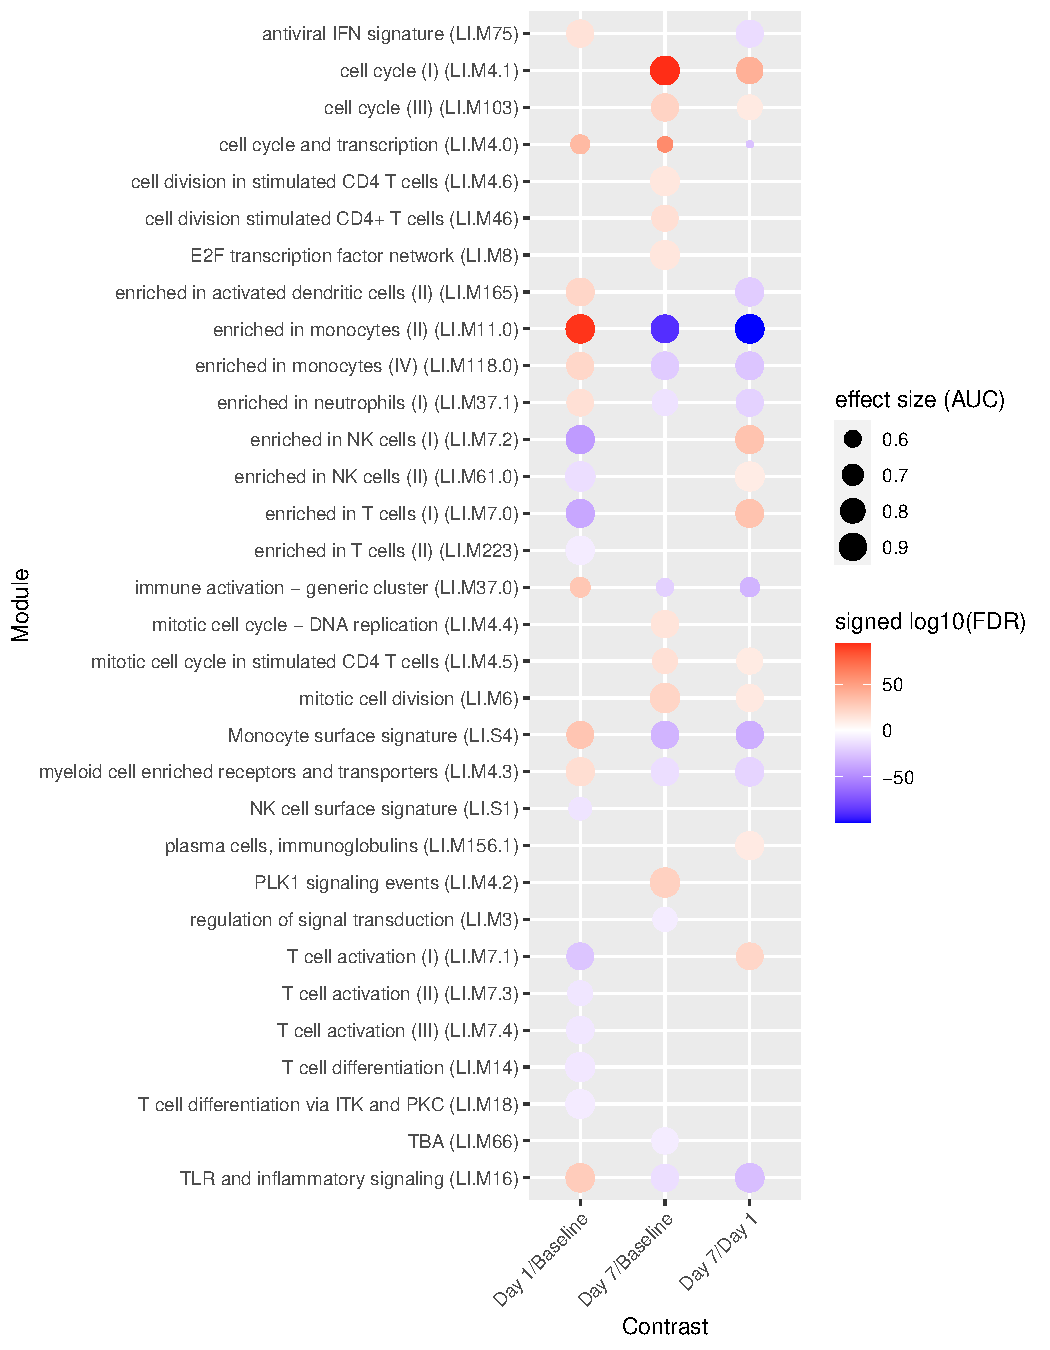
\includegraphics[width=1.0\textwidth]{mainmatter/figures/chapter_02/compare_dge_eqtl.tmodDotPlot.DGE.timepoint.pdf}
    \caption{Transcriptomic modules significantly up or downregulated post-vaccination. Size of circle indicates effect size. Color of circle indicates significance and direction of effect (red = upregulation, blue = downregulation).}
    \label{fig:hird_tmodDotPlot_timepoint}
\end{figure}
\todo{change x axis labels to baseline, specify top 10 procedure in figure caption}

\subsection{Adaptive immune response at day 7 post-vaccination}

59 genes were differentially expressed at day 7 vs. baseline, with expression fold changes more modest than those at day 1.
The genes with the highest upregulation were the B cell-associated genes \gene{TNFRSF17} ($\log_2\text{\gls{FC}} = 1.7538617$) and \gene{MZB1} ($\log_2\text{\gls{FC}} = 1.7369668$).
Plasma cell-specific genes including \gene{SDC1} (encodes CD138 \url{https://www.ncbi.nlm.nih.gov/pmc/articles/PMC5437827/}) ($\log_2\text{\gls{FC}} = 1.3673081$) and \gene{ELL2} (\url{https://www.nature.com/articles/ni.1786}) ($\log_2\text{\gls{FC}} = 0.8679659$) were also prominently upregulated.
\todo{finish citing}
Strongly enriched modules at day 7 were related to mitosis and cell proliferation, particularly in CD4\textsuperscript{+} T cells (\autoref{fig:hird_tmodDotPlot_timepoint}).
Both the CD4\textsuperscript{+} T cell and plasma cell response are indications of an adaptive immune response at day 7.

\subsection{Expression signatures associated with antibody response}

I also looked for genes which have expression associated with baseline-adjusted antibody response, as quantified by \gls{TRI}.
At the initial frequentist meta-analysis stage, with a significance threshold of $\text{\gls{FDR}} < 0.05$, 6 genes had expression associated with \gls{TRI} at baseline, 55 at day 7, and 11 pooling samples across timepoints (\autoref{fig:hird_DGE_effectSizeComparisons_rma}).
\autocite{sobolev2016AdjuvantedInfluenzaH1N1Vaccination} also identified genes with day 7 expression associated with antibody response, where response was defined as a binary phenotype based on 4-fold change (described in section \todo{add label}).
They reported 62 significant associations at \gls{FDR} $< 0.05$, of which 58/62 fall into the 13593 genes considered in my meta-analysis (circled, \autoref{fig:hird_DGE_effectSizeComparisons_rma}), and 15/58 replicated, all with the same positive direction of effect (high expression with high \gls{TRI}).
In the Bayesian meta-analysis, no single gene was detected as significantly associated with \gls{TRI} at $\text{\gls{lfsr}} < 0.05$ at any timepoint, or when pooling samples across all timepoints (\autoref{fig:hird_DGE_effectSizeComparisons_bayesmeta}).

\begin{figure}
    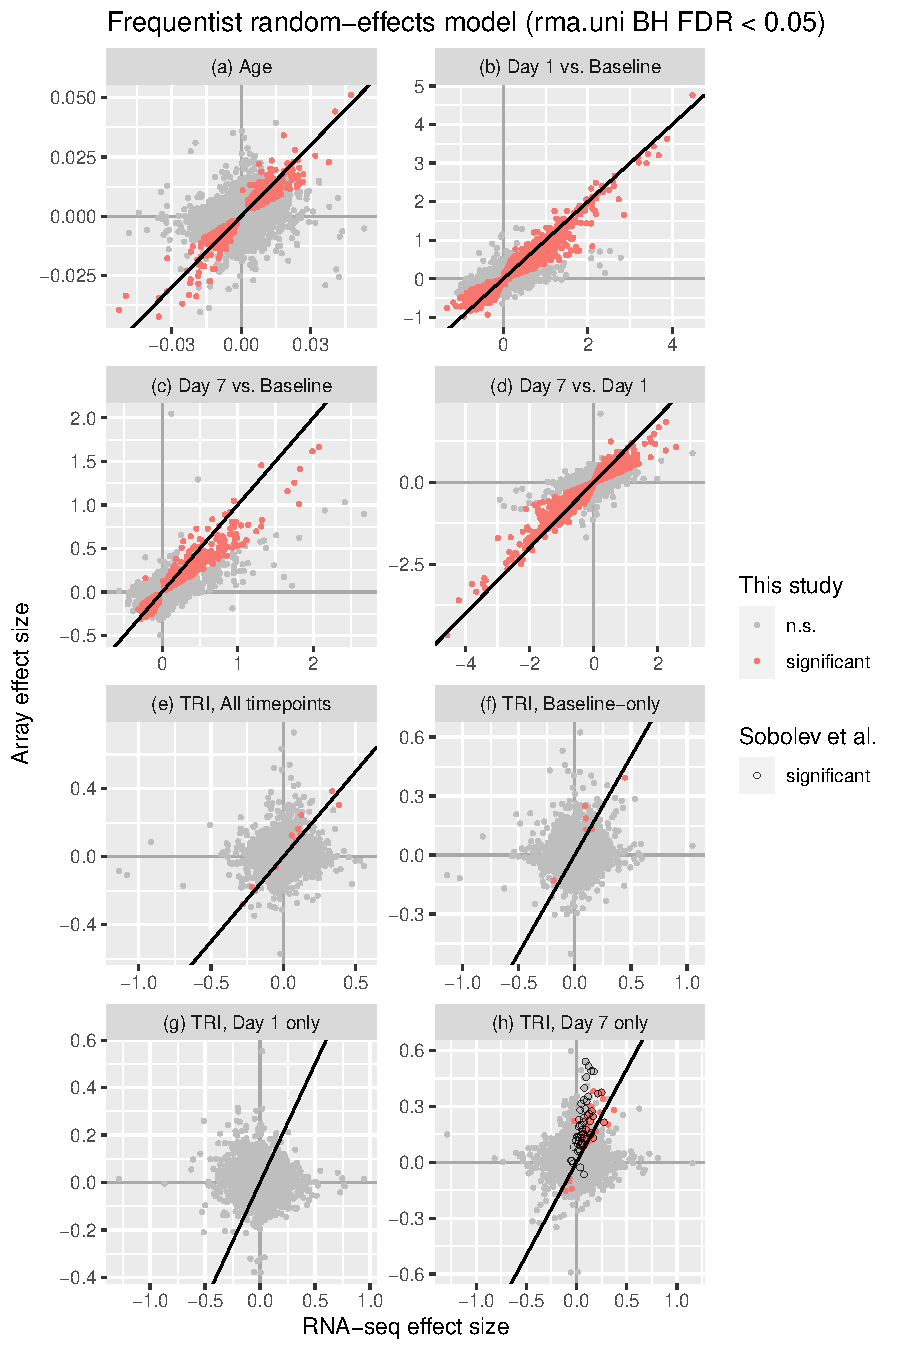
\includegraphics[width=1.0\textwidth,page=1]{mainmatter/figures/chapter_02/plot_dge_eqtl.DGE.effectSizeComparison.pdf}
    \caption{DGE effect sizes estimated in array vs. \gls{RNAseq}. Significance colored by frequentist random effects meta-analysis FDR < 0.05. Genes with day 7 expression associated with responder/non-responder status in \autocite{sobolev2016AdjuvantedInfluenzaH1N1Vaccination} are circled for that contrast.}
    \label{fig:hird_DGE_effectSizeComparisons_rma}
\end{figure}

\begin{figure}
    \includegraphics[width=1.0\textwidth,page=2]{mainmatter/figures/chapter_02/plot_dge_eqtl.DGE.effectSizeComparison.pdf}
    \caption{DGE effect sizes estimated in array vs \gls{RNAseq}. Significance colored by Bayesian random effects meta-analysis lfsr < 0.05. Genes with day 7 expression associated with responder/non-responder status in \autocite{sobolev2016AdjuvantedInfluenzaH1N1Vaccination} are circled for that contrast.}
    \label{fig:hird_DGE_effectSizeComparisons_bayesmeta}
\end{figure}

Significant enrichments were detected at the gene set level; the strongest effects are seen at day 7, where expression of cell cycle, CD4\textsuperscript{+} T cells, and plasma cells are associated with high \gls{TRI}.
At day 0, modules related with inflammatory response in myeloid cells are also associated with high \gls{TRI} (\autoref{fig:hird_tmodDotPlot_TRI}).

\begin{figure}
    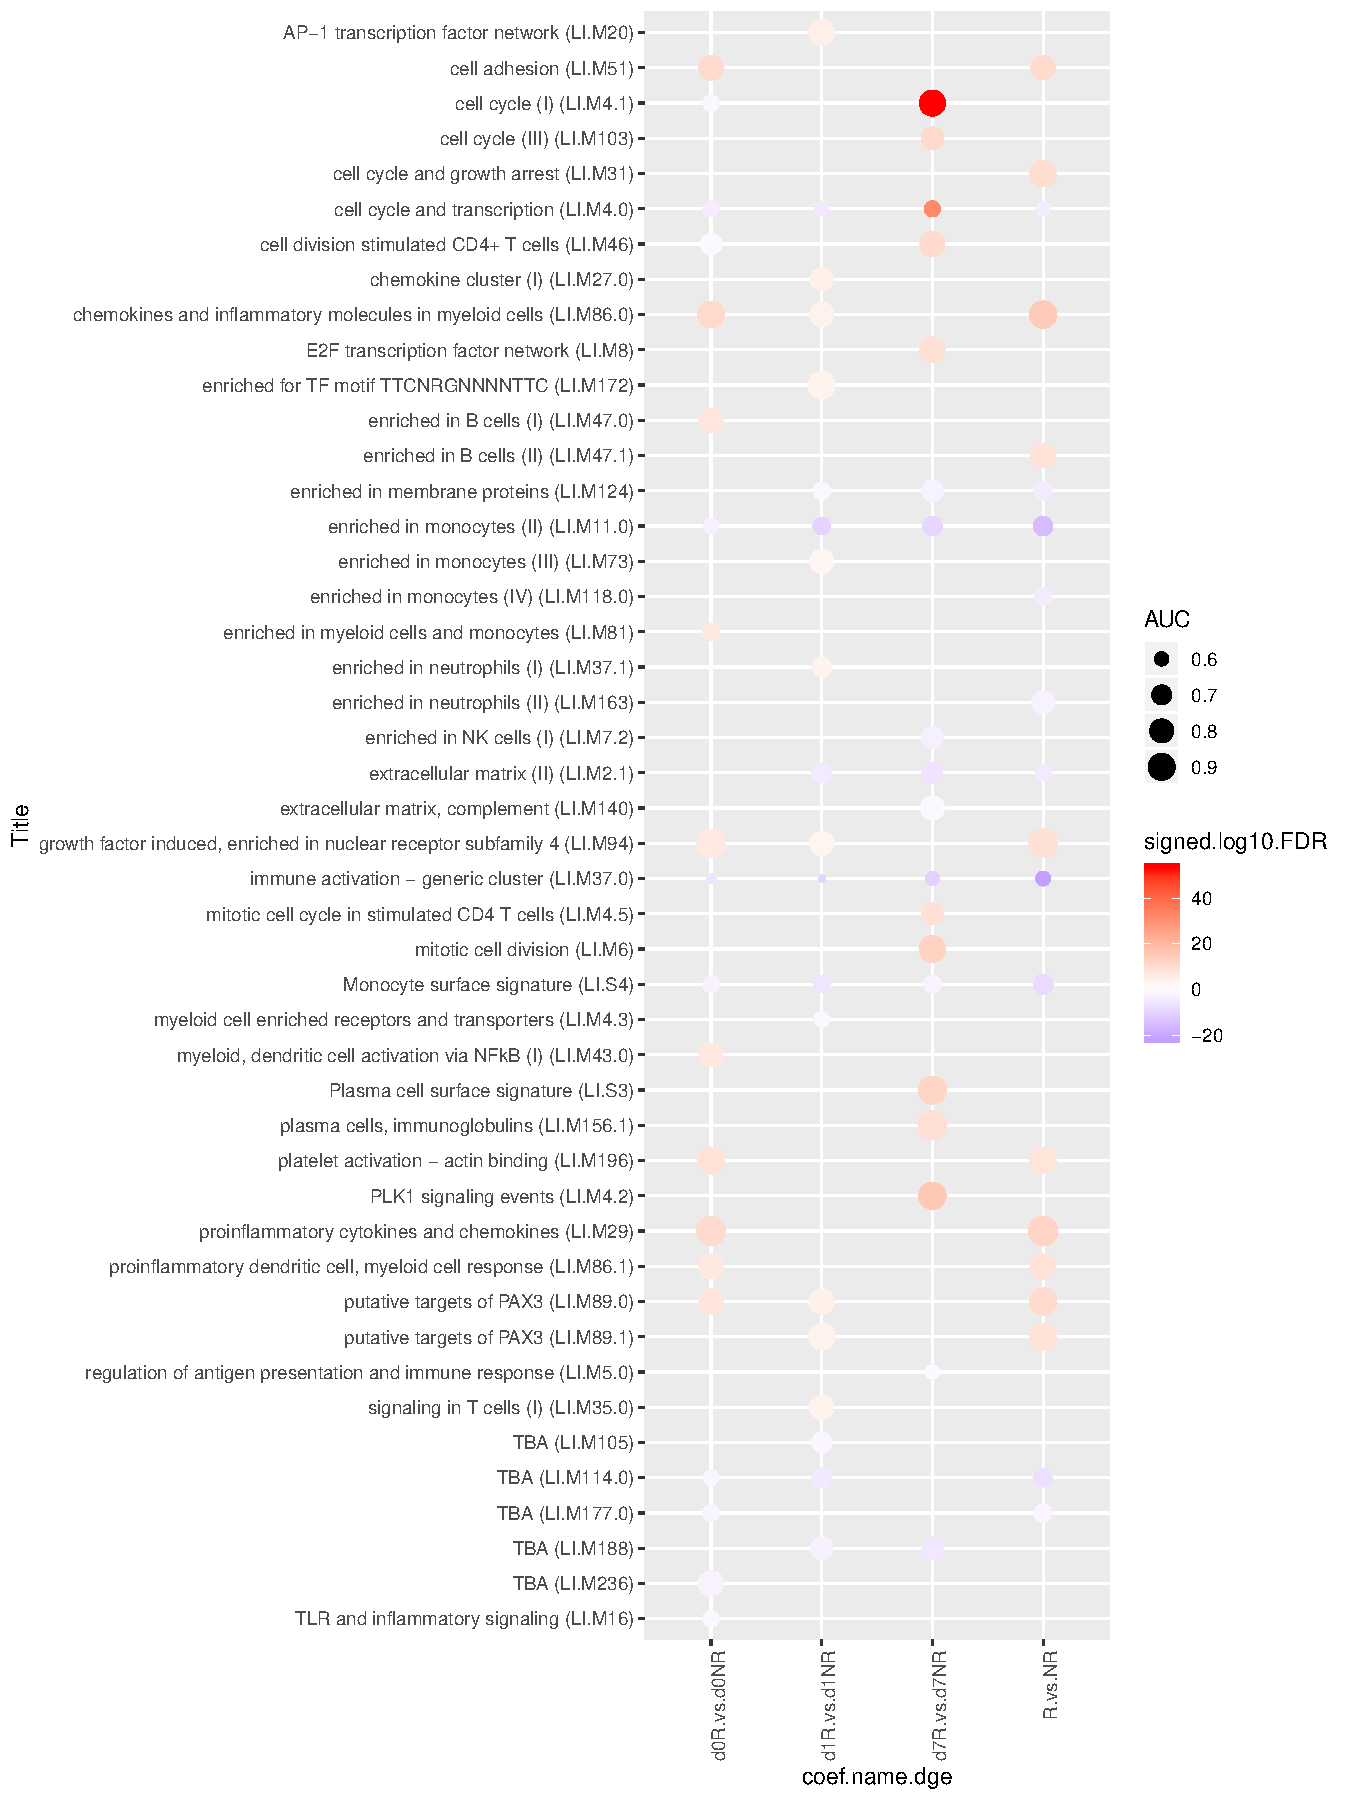
\includegraphics[width=1.0\textwidth]{mainmatter/figures/chapter_02/compare_dge_eqtl.tmodDotPlot.DGE.TRI.pdf}
    \caption{Transcriptomic modules enriched in genes with expression associated with antibody response (\gls{TRI}) at each day. Size of circle indicates effect size. Color of circle indicates significance and direction of effect (red = expression positively correlated with TRI, blue = negative).}
    \label{fig:hird_tmodDotPlot_TRI}
\end{figure}
\todo{figure x labels here should be TRI, not R.vs.NR}

\subsection{Identifying expression signatures for predicting antibody response [probably cut this section and just add to discussion]}

\section{Discussion}

There is extensive transcriptomic response to Pandemrix vaccination in the \gls{HIRD} cohort.
Upregulation of genes and modules related to the interferon signalling pathway, monocytes, inflammatory response, and other aspects of innate immunity were detected at day 1.
This response is transient, with most such genes returning to baseline expression by day 7.
\todo{Not sure if there is a biological interpretion of downreg of T cells and NK cells gene sets at day 1, since it could be due to increase in other cell types in the sample. similar findings in \autocite{nakaya2016SystemsBiologyImmunity} though}
\todo{lit search for downregulation interpretation paper, and downreg T cell paper}
% TODO: TMM norm guards this
Upregulation of cell cycle/proliferation, activated CD4\textsuperscript{+} T cell, and B (plasma) cell genes and modules were detected at day 7.
This is likely a signature indicating the shift to an adaptive immune response, involving CD4\textsuperscript{+} T cell-supported differention and proliferation of antibody-secreting plasmablasts and plasma cells\autocite{murphy2016JanewayImmunobiology}.
These patterns of expression change between timepoints in the \gls{RNAseq} data are consistent with the patterns in the array data in the original study\autocite{sobolev2016AdjuvantedInfluenzaH1N1Vaccination}, and with expansions of monocyte and plasma cell populations seen in the \gls{FACS} data at days 1 and 7 respectively in the original \gls{HIRD} study\autocite{sobolev2016AdjuvantedInfluenzaH1N1Vaccination}.

In contrast, I was not able to fully replicate the originally reported single gene-level associations between day 7 expression and antibody response in the \gls{RNAseq} data and subsequent and meta-analyses.
In \autocite{sobolev2016AdjuvantedInfluenzaH1N1Vaccination}, 62 genes were reported as differentially expressed between vaccine responders and non-responders.
Although \autocite{sobolev2016AdjuvantedInfluenzaH1N1Vaccination} encodes responder status as a binary phenotype, whereas my analysis uses \gls{TRI}, this is not the primary difference, as 51/62 genes replicated (\gls{FDR} < 0.05) using \gls{TRI} when considering just the array data.
The same analysis using only the \gls{RNAseq} data replicated 0/62 genes.
\todo{might have to rerun everything using the original binary R/NR if this line of reasoning isn't strong enough}
\todo{move numbers to results?}
The majority of the effects for these genes were simply much stronger in the array dataset than in the RNAseq dataset (\autoref{fig:hird_DGE_effectSizeComparisons_rma}).
Given that the range of \gls{TRI} is higher in the array individuals (\autoref{tab:hird_table1}), this does not seem unusual that stronger \gls{TRI}-associated effects are observed there.
%
% \todo{TRI (cite) is a bit of a hack too to combine two assays. it seems to be 'residualised change score'}
% lots of issues in lit, see ch3 section
% \todo{also, see sorjonen2019PerilAdjustingBaseline change as predictor}
% should probably analyse MN, HAI, separately after log

58/62 reported hits were measured by both platforms and assessed in the meta-analysis.
Only 15/58 signals replicated using frequentist random-effects meta-analysis to combine per-platform estimates.
I do not consider these hits as robust, as the \gls{REML} estimate of between-platform heterogeneity was zero for 8563/13593 for the day 7 TRI contrast overall, and zero for all 15 of these signals.
None of these signals replicated in the Bayesian random-effects meta-analysis.
The Bayesian meta-analysis is in general more conservative, calling fewer differentially expressed genes compared to the frequentist analysis for all contrasts (\autoref{fig:hird_DGE_effectSizeComparisons_bayesmeta}).
Prior information about $\tau$ is incorporated, discouraging unrealistic estimates of zero heterogeneity.
Given the between-platform heterogeneity coming from both platform-specific technical differences and \gls{TRI} phenotype differences, relative to the modest effect size distributions compared to between-timepoint \gls{DGE} comparisons, the data are not well-positioned to identify significant single-gene associations with antibody response.
%
% Other caveats of the meta analysis
% - The very fact that a meta-analysis is performed adds some bias towards genes with fold changes that can be more consistently measured between platforms; these tend to be genes with higher expression.

% Did we choose the right phenotype?
%
% - the day 63 timepoint is late compared to many other studies
% - Nauta JJ, Beyer WE, Osterhaus AD. On the relationship between mean antibody level, seroprotection and clinical protection from influenza. Biologicals 2009; 37:216-21; PMID:19268607; http://dx. doi.org/10.1016/j.biologicals.2009.02.002 "In clinical studies seroprotection is normally defined as a specific antibody titer or antibody titer increase (seroconversion)."
% - other measures of seroconversion \url{https://www.who.int/biologicals/vaccines/Annex_2_WHO_TRS_963-3.pdf}
% - https://bmcinfectdis.biomedcentral.com/articles/10.1186/s12879-019-4049-5 Seroconversion may not correspond well to protection...

Expression signatures of antibody response were, however, observed at the gene set level, for modules of coexpressed genes that are associated with \gls{TRI} as a whole.
The strongest effects were observed at day 7, where expression of adaptive immune response modules (cell cycle, stimulated CD4\textsuperscript{+} cell, plasma cell modules) were positively associated with \gls{TRI}.
These are the same modules observed to be upregulated at day 7 compared to baseline; it seems that those individuals with the greatest antibody response to vaccination are most able to upregulate these gene sets by day 7 post-vaccination.

Module associations were also observed pre-vaccination (cell adhesion, enriched in B cells, proinflammatory cytokines, platelet activation), suggesting baseline immune state has some influence on long-term antibody response to Pandemrix.
%
% Day 1 TRI ?
% Inflammatory signatures of non-response
% https://www.jacionline.org/article/S0091-6749(17)31766-9/fulltext#sec2.4
% \enquote{The reduced efficacy of vaccination has also been linked to excessive inflammation for influenza,31 yellow fever,32 tuberculosis,33 and hepatitis B34 vaccines.}
%
Over the years, a diverse range of gene sets have been found to be baseline predictors of serological response to influenza vaccination:
    apoptosis\autocite{furman2013ApoptosisOtherImmune}; 
    Fc$\gamma$ receptor-mediated phagocytosis, TREM1 signaling\autocite{tsang2014GlobalAnalysesHuman};
    enriched in B cells, T cell activation\autocite{nakaya2015SystemsAnalysisImmunity};
    B cell receptor signalling, inflammatory response, platelet activation \autocite{hipc-chisignaturesprojectteam2017MulticohortAnalysisReveals}; 
several of which I also observe.
It should be noted that comparisons with these signatures from existing influenza systems vaccinology studies should caveated, as most existing studies are for non-adjuvanted influenza vaccines.
Adjuvanted influenza vaccines are considerably more immunogenic, and post-vaccination expression patterns differ to those of non-adjuvanted vaccines \autocite{sobolev2016AdjuvantedInfluenzaH1N1Vaccination,wilkins2017AS03MF59AdjuvantedInfluenza}.
\todo{could comment on phenotype differences too, i.e. HIRD measure antibodies at d63, much later than is popular in the field: d28 usually}
\todo{should probably emph sobolev didn't find prevacc signatures, and we did. But it's not exactly fair, as sobolev didn't use gene set enrichment as far as i can tell}
Hence, it is particularly important that the robustness of these observed baseline expression signatures be validated in an independent cohort for a comparable AS03-adjuvanted influenza vaccine.

%
% Sobolev:
% Of the volunteers analyzed, essentially all showed expansive changes in peripheral blood gene expression by day 1 (significant changes in ~9,000 gene probes (P < 0.05)) (Supplementary Fig. 2a), highly consistent with other studies that did not use adjuvants8,16,24,25.
% [...]
% In that regard, our study shows that the Pandemrix H1N1 vaccine provokes rapid and expansive, yet transient, activation of myeloid cells and effectors, similarly to changes induced by other vaccines, including flu vaccines lacking adjuvant8,13,15–17. However, our study also reveals a pronounced lymphoid contribution to the early phase of the immune response, most evident in the prominent transient upregulation of IFN-γ, which was not apparent in most other virus vaccine studies.
%
% As noted by \autocite{sobolev2016AdjuvantedInfluenzaH1N1Vaccination}, although the day 1 myeloid response was consistent with studies of non-adjuvanted seasonal influenza vaccines (e.g. \autocite{nakaya2011SystemsBiologyVaccination, bucasas2011EarlyPatternsGene, obermoser2013SystemsScaleInteractive}), the presence of interferon gamma-driven responses was unique to \gls{HIRD}.
% \todo{I think i did not mention specifically type II (IFN-g) in the results section. would need to add HALLMARK set CAMERA results to show this}
%
% Although it is known that AS03 does induce expression changes related to innate immune response at the injection site (\url{https://www.sciencedirect.com/science/article/pii/S0264410X11000399?via%3Dihub#sec0010}), the mechanism of action is unknown (\url{https://www.frontiersin.org/articles/10.3389/fimmu.2017.01760/full}), and there have been relatively few studies of the effect of AS03 or AS03-adjuvanted vaccines on the \gls{PBMC} immune transcriptome aside from the \autocite{sobolev2016AdjuvantedInfluenzaH1N1Vaccination} study itself.
%
% https://www.sciencedirect.com/science/article/pii/S1879625711000769?via%3Dihub#bib0180
% Their mechanism of action remains incompletely understood, however they may amplify immune responses by enhancing antigen presentation and recruiting inflammatory cells to the area of antigen deposition (reviewed in [36]).
%
% https://link.springer.com/article/10.1007/s10875-010-9490-6
% Immune responses to inactivated influenza virus adjuvanted with a different oil-in-water emulsion, MF59, have recently been described [35, 36]. Although a direct comparison between the adjuvants is complicated by the fact that different methodologies may have been used to measure immune responses, our data indicate that AS03A-adjuvanted influenza vaccines induce strong HI responses and CD4 T-cell frequencies relative to those induced with the MF59-adjuvanted product.
%
% AS03-adjuvanted split-virion influenza A/H5N1 vaccine: (\gene{GBP1}, \gene{IRF1}, and \gene{STAT1}) expressions are up in adjuvanted (\url{https://journals.plos.org/plosone/article?id=10.1371/journal.pone.0167488}), three genes that play a role in interferon and antiviral response.
%
% A study of the MF59-adjuvanted \gls{TIV} \autocite{nakaya2016SystemsBiologyImmunity}
%

% TODO: prediction will be discussed in ch5
%
% Sobolev:
% In sum, neither molecular nor cellular data offered any consensus prevaccination predictor of nonresponsiveness akin to those proposed in studies of nonadjuvanted vaccines8,16,17,24,31.
%
% We find some, but...
% - The utility of such signatures is unclear.
% - diagnostics would require prediction
% - and would require protection, not immuno
%
% TODO
% \todo{There is also something to be said about 'prediction is not inference'. For use as correlates of protection, as promised by proponents of systems studies, prediction is what is important.}
% TODO: i have defined what would be deemed "correlates of ab response", now move to prediction

% Seasonal can prime for H1N1
%
% \2 Efficacy, dosing: \enquote{...a single dose of monovalent 2009 H1N1 vaccine was recommended in adults, but young children were recommended to receive 2 doses (reviewed by [3••]). It is likely that a single dose was sufficient to induce immunity in adults because prior exposure to seasonal H1N1 viruses had immunologically primed the population.}
%
% "Seasonal influenza vaccine provides priming for A/H1N1 immunization." \url{https://www.ncbi.nlm.nih.gov/pubmed/20371459}
%
% Demonstration in a mouse model: \url{https://www.ncbi.nlm.nih.gov/pmc/articles/PMC3024675/}
%
% \2 Inclusion of H1N1 strains into seasonal vaccines
% Sobolev sampled in March 2010 to August 2011
% \2 Later cohorts may have recall response to H1N1 from seasonal vaccination

% TODO: compare to seasonal

% - Overall conclusions.
In conclusion, Chapter 2 characterises the expansive changes in \gls{PBMC} gene expression that follow vaccination with Pandemrix.
The dominant trend for all individuals is transient upregulation of the innate immune response at day 1, transitioning into adaptive immunity by day 7.
Baseline-adjusted antibody response is correlated with expression of gene sets, particularly adaptive immunity modules at day 7, but also for some modules pre-vaccination.
Unfortunately, between-platform variation in expression impedes identification of specific genes that contribute.
The fundamental question of why gene expression and antibody responses vary between \gls{HIRD} individuals remains.
Chapter 3 will examine one hypothesis: the impact of common human genetic variation on Pandemrix expression response.
% TODO: ch4 also corrects for cell props
\todo{At no point in this chapter are we estimating causal effects: add point on why not CIT (lower n than franco)}
\todo{found signatures, but so what? Feels like chapter lacks a punchline?}

% TODO: not adjusted for cell comp, but not necc bad
% in ch4, I adjust

% TODO: add a whilst we were not able to X in the intro, the field has advanced by Y, future Z needed

% TODO: beyond 28d Ab tites: Influenza vaccine–induced human bone marrow plasma cells decline within a year after vaccination \url{https://science.sciencemag.org/content/early/2020/08/12/science.aaz8432}
% were not able to explore actual protectiveness

% TODO:
% also need the cellular response, beyond ab titires cao2016SystemsImmunologyAntibody
